% !TeX spellcheck = pt_BR

\chapter{Introdução} \label{chapter_intro}



Um número enorme de estudantes conclui seus estudos de física no ensino médio com a leve sensação de que tudo funciona quase como uma espécie de mágica. Tem-se uma quantidade enorme de fórmulas --- que sabe-se lá de onde vieram ou por que funcionam --- que devem ser memorizadas e, ao acertar qual é a fórmula correta a se usar em um certo contexto, jogam-se os valores, fazem-se algumas contas, e \textit{voilà}: a resposta sai ao final, como em um passe de mágica.

Talvez a sensação de que tudo seja um grande truque de mágica deva-se ao fato de que nunca se entende muito bem as tais fórmulas, de modo que questionamentos acabam surgindo. Mas, na maior parte das vezes, não costumam ser bem recebidos da parte de quem ministra as aulas:

\begin{center}
  \textit{De onde essas fórmulas vieram? Por que funcionam? Por que foram criadas? Aliás...elas foram criadas? E por qual motivo temos que estudar isso?}
\end{center}

Se você já se fez alguma dessas perguntas, ou se alguma delas lhe despertou o interesse, a jornada que iniciaremos agora lhe soará como um belo e prazeroso passeio. Vamos, portanto, começar.


\section{De onde vem a fórmula, afinal?}

Talvez o primeiro questionamento que devemos tentar responder seja:

\begin{center}
    \textit{O que exatamente é uma fórmula de física?}
\end{center}


Para tentar entender isso, vamos começar com o problema de transmitir uma informação. Digamos que eu queria transmitir ao leitor a informação contida na Figura \ref{intro01}.

\begin{figure}[h]
    \centering
    \begin{tikzpicture}
      \begin{scope}[blend mode=multiply]
        \node {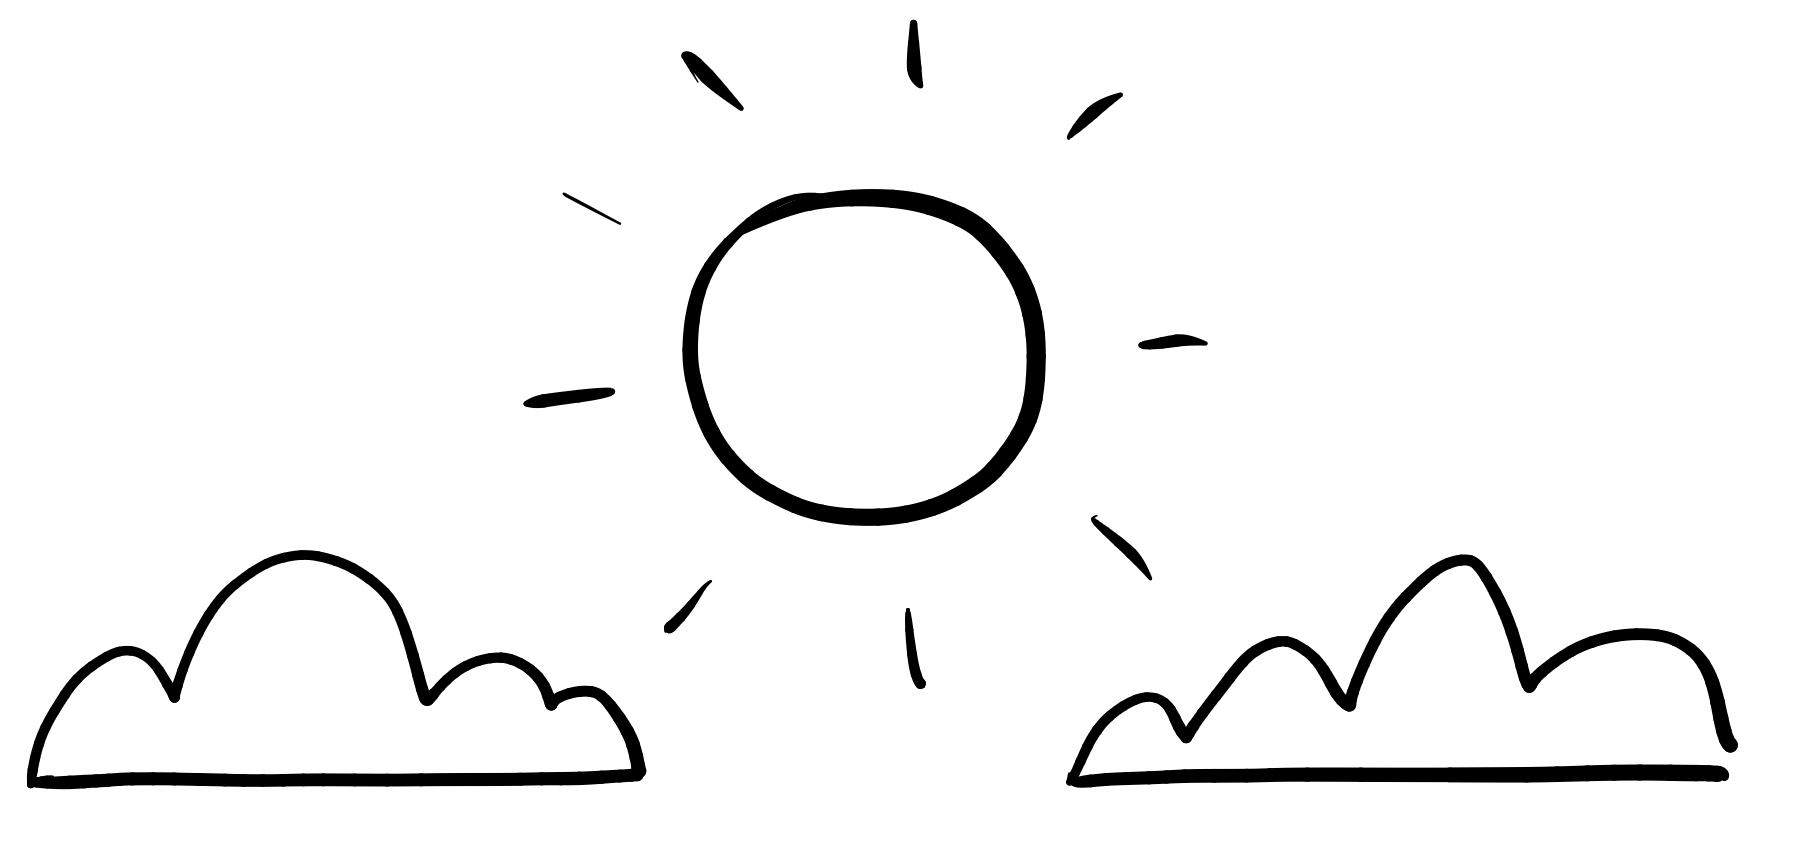
\includegraphics[scale=0.09]{imagensintro/sol.jpeg}};
      \end{scope}
    \end{tikzpicture}
    \caption{Uma figura qualquer.}
    \label{intro01}
\end{figure}

Existem algumas opções disponíveis: a primeira delas é simplesmente mostrar-lhe a imagem, que carrega toda a informação que preciso te transmitir. A segunda, talvez, seria descrever-lhe, em palavras, o que está representado na figura. Algo como: imagine um sol com duas nuvens abaixo. 

Ou então, eu poderia também lhe passar a seguinte informação: 

\begin{center}
    \begin{otherlanguage}{greek}
Φανταστείτε έναν ήλιο με δύο σύννεφα από κάτω του.
\end{otherlanguage}
\end{center}


Talvez isso lhe pareça grego e você não tenha entendido nada --- se foi o caso, bem, isso é grego mesmo. Acontece que, no fundo, a Figura \ref{intro01}, a frase ``\textit{imagine um sol com duas nuvens abaixo}'' ou a informação aparentemente criptografada \begin{otherlanguage}{greek} Φανταστείτε έναν ήλιο με δύο σύννεφα από κάτω του \end{otherlanguage} representam exatamente a mesma coisa, são apenas linguagens diferentes para expressar uma mesma informação. A frase em grego parece um amontoado de símbolos desconexos pelo simples fato de que você desconhece essa linguagem. Talvez, inclusive, você tenha se precipitado a julgar que essa última forma é a mais complicada, mas certamente um grego discordaria de você. A melhor linguagem para expressar essa informação, para um grego, certamente seria a última. Ou talvez a primeira, a do desenho, que parece ser uma linguagem mais universal --- se bem que um cego certamente discordaria disso.

Note que a melhor linguagem para expressar a informação, neste caso, depende de quem a recebe. A informação se expressa melhor em português para brasileiros, em grego para gregos, em mandarim para chineses...

O que buscamos é uma forma universal e mais adequada para expressar algumas informações a respeito dos fenômenos da natureza: é isso que a física se propõe a fazer.

Digamos, para exemplificar isso, que fizemos o seguinte experimento: soltamos uma pedra do alto de um prédio, e um instrumento de medida nos permite perceber que a pedra percorre, a cada segundo, distâncias que estão na proporção dos números ímpares: 1,3,5,7,9...

\begin{figure}[h]
    \centering
    \begin{tikzpicture}
      \begin{scope}[blend mode=multiply]
        \node {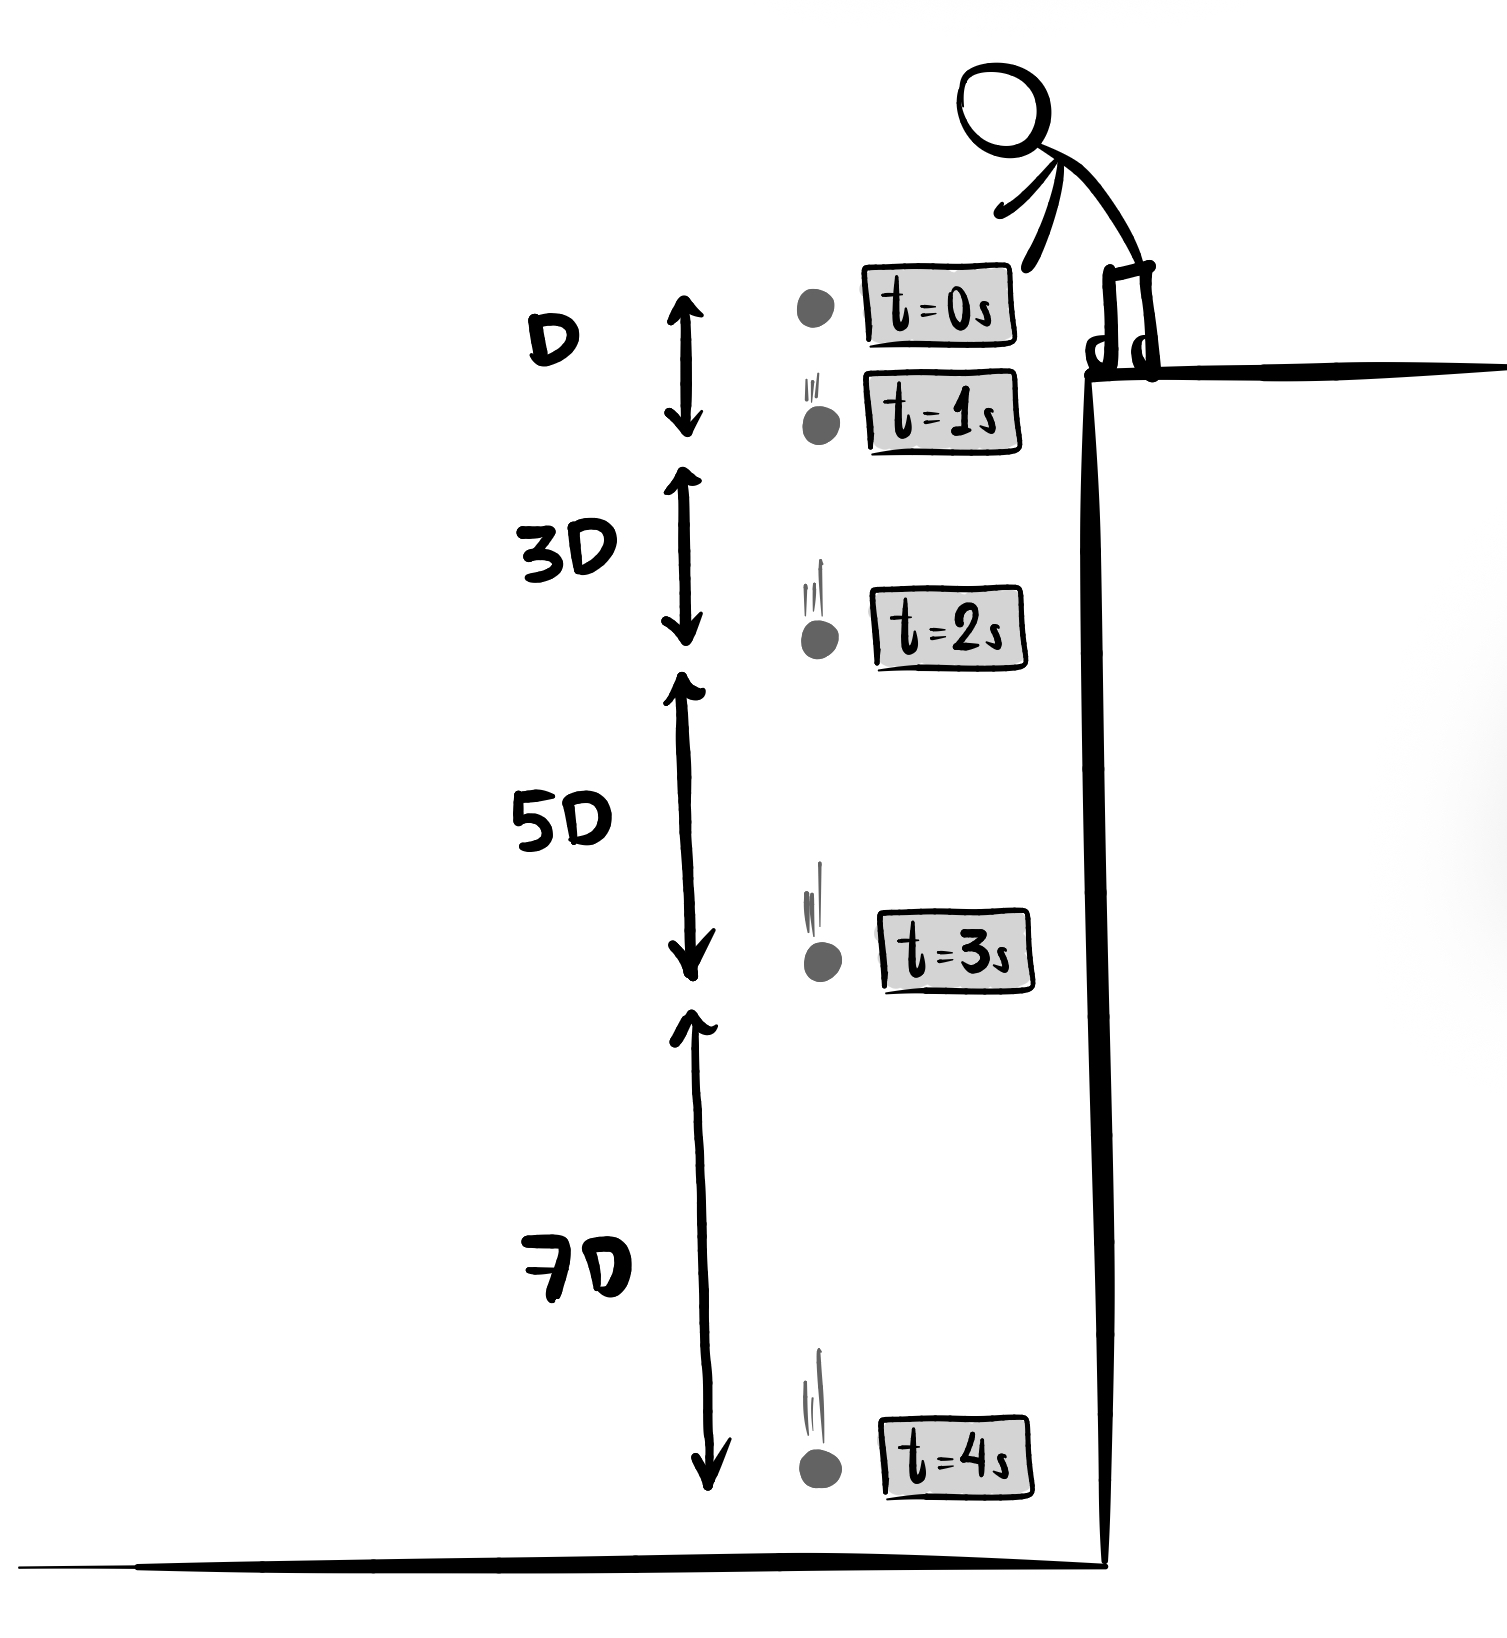
\includegraphics[scale=0.16]{imagensintro/quedalivre.jpeg}};
      \end{scope}
    \end{tikzpicture}
    \caption{Tentando novamente transmitir informações por meio de um desenho.}
    \label{intro02}
\end{figure}

Uma forma de te transmitir o resultado deste experimento é te entregando um desenho como o da Figura \ref{intro02}, que tenta sintetizar o que foi feito e qual foi o resultado obtido. Alguém poderia alegar que nem todos poderiam extrair de tal desenho exatamente o que seria necessário, por mais que o autor tenha colocado empenho e dedicação em fazer um bom desenho que fosse o mais fiel possível ao experimento realizado. Uma outra forma, talvez mais objetiva e que evite ambiguidade, seria dizer que

\begin{center}
    \textit{Ao fazer o experimento de abandonar uma pedra do repouso e deixá-la cair\footnote{Sem resistência do ar.}, nota-se que as distâncias percorridas em intervalos de tempo iguais e sucessivos estão na proporção dos números ímpares.}
\end{center}

Talvez isso lhe pareça ainda um pouco confuso --- e certamente poderíamos ter dado um jeito de expressar isso em língua portuguesa de forma mais clara --- mas essa foi exatamente a forma como Galileu Galilei, no século XVII, enunciou a chamada lei da Queda Livre, ao realizar tal experimento.

Um outro modo de sintetizar a mesma informação é dizendo que, sendo $s$ a distância vertical que a pedra percorre a partir do repouso (do ponto em que ela é abandonada) e sendo $t$ o tempo de movimento, contado a partir do instante em que a pedra é abandonada, então

\begin{equation}
    s = kt^2,
    \label{00intro_eq_quedalivre}
\end{equation}
em que $k$ é alguma constante.

Talvez a Equação \eqref{00intro_eq_quedalivre} soe, para o leitor, tão grego quanto a frase em grego anteriormente citada. Se este é o caso, tudo bem: não espero que você, a essa altura, tenha compreendido tudo.\footnote{Para o leitor mais afoito e curioso, note que em $t=1$ teríamos $s=k$; em $t=2$ teríamos $s=4k$; em $t=3$ teríamos $s=9k$; e por aí vai. Para avaliar a distância que a pedra percorre em intervalos \textbf{sucessivos} de tempo, teríamos que pegar a diferença entre suas posições em instantes consecutivos de tempo, isto é, a distância percorrida no segundo entre $t=1$ e $t=2$ seria a diferença entre $4k$ e $k$, ou seja, $3k$. A distância percorrida no segundo entre $t=2$ e $t=3$ seria a diferença entre $9k$ e $4k$, ou seja, $5k.$ Percebeu de onde surgem os números ímpares?} Contudo, é preciso notar que, até aqui, temos, a princípio, três formas de exprimir a informação a respeito do que observamos em nosso experimento:

\begin{itemize}
    \item [(i)] Por meio de um desenho, como o da Figura \ref{intro02}.

    \item [(ii)] Por meio da língua portuguesa (ou do grego, para gregos; ou mandarim, para chineses) em uma frase como

\begin{center}
    \textit{Ao fazer o experimento de abandonar uma pedra do repouso e deixá-la cair, nota-se que as distâncias percorridas em intervalos de tempo iguais e sucessivos estão na proporção dos números ímpares.}
\end{center}

  \item [(iii)] Por meio de uma fórmula matemática, como a Equação \eqref{00intro_eq_quedalivre}.
    
\end{itemize}



A primeira forma certamente possui suas limitações: um desenho é algo um pouco subjetivo e pode dar margem para interpretações equivocadas ou ambiguidades, por melhor e mais detalhado que ele tenha sido feito. Entre as formas $(ii)$ e $(iii)$ de se exprimir a informação, o leitor --- por mais que não compreenda como a equação $s=kt^2$ contém a informação de que as distâncias percorridas em intervalos de tempos iguais estão na proporção dos números ímpares --- há de concordar que o caminho $(iii)$ é superior: ele é o mais sucinto de todos. Por mais que a este momento lhe pareça grego, se você acreditar que a Equação \eqref{00intro_eq_quedalivre} contém toda a informação a respeito do resultado do experimento, você terá que concordar que, expressar tudo isso usando apenas 3 letras, 1 número e 1 caractere especial (o símbolo de igualdade) como tal equação faz é algo extremamente sofisticado. E melhor: não precisa de tradução. Pelo caminho $(ii)$ nós teríamos que traduzir para o grego, para o mandarim ou para algum outro idioma caso a conversa fosse com um estrangeiro. Já o caminho $(iii)$ não: ele é uma linguagem universal. Desde que se entenda tal linguagem --- a matemática --- um grego, um brasileiro, um chinês ou um russo seriam capazes de compreender e extrair a informação a respeito de como a natureza funciona ao soltarmos uma pedra do alto de um prédio.

Com isso, o leitor deve ter compreendido agora o que é uma fórmula de física: é uma forma de se expressar, por meio da linguagem matemática, uma informação.\footnote{É por isso que alocar energia para memorizar uma fórmula, sem compreender qual é a informação que ela se propõe a sintetizar, é uma grande perda de tempo. O foco deve estar sempre em compreender a informação e, posteriormente, entender como e por que tal fórmula matemática a sintetiza. É o que faremos nessa jornada.} Tal informação pode ser o resultado de um experimento, por exemplo, e ela poderia muito bem ser expressa por meio da língua falada, de um desenho ou de algum outro método qualquer --- todas essas outras formas são, contudo, bem menos eficientes, como já argumentamos.

Acontece que o terceiro caminho --- expressar o resultado de como a natureza se comporta por meio de uma fórmula matemática --- é superior a todos os demais por um outro fato: a natureza revela os seus padrões por meio da matemática. Por que isso ocorre, ninguém sabe muito bem \footnote{Inclusive, um grande físico, Eugene Wigner, vencedor do prêmio Nobel de Física de 1963, escreveu um artigo famoso intitulado \textit{The Unreasonable Effectiveness of Mathematics in the Natural Sciences} , em que ele concluiu que o fato de a matemática funcionar de modo extremamente eficaz para explicar a natureza é algo inexplicável, quase um milagre.} Mas o fato é que isso ocorre, e foi percebido pela primeira vez possivelmente por Galileu, que escreveu que

\begin{quote}
    A filosofia (isto é, a ciência) está escrita neste grandíssimo livro que, continuamente, está aberto diante de nossos olhos (eu quero dizer o universo), mas que não se pode entender se não se aprende a entender a língua, e a conhecer os caracteres, nos quais está escrito. Ele é escrito em língua matemática, e os caracteres são os triângulos, círculos, e outras figuras geométricas, sem cujos meios é humanamente impossível entender uma só palavra; sem esses é um vão caminhar por um obscuro labirinto.
\end{quote}


Ora, se a natureza não fala por palavras, mas sim por relações matemáticas, as equações são o modo mais honesto e eficiente que encontramos para escutá-la, estudá-la e compreendê-la. Para concluir essa introdução, espero que até aqui tenha ficado claro para o leitor: \textbf{uma fórmula de física é simplesmente um meio de se expressar, matematicamente, uma informação a respeito da natureza. Tal forma é a mais eficiente e objetiva, uma vez que a natureza se expressa em linguagem matemática.} Cabe destacar que, por meio da linguagem matemática, torna-se possível mensurar e transmitir informações quantitativas de forma mais precisa. Por exemplo, no contexto da Figura \ref{intro01}, é possível, por meio de uma equação matemática, expressar --- por meio de grandezas físicas adequadas --- o quão quente estava aquele dia ou o quão brilhante estava o sol, informações estas que seriam difíceis de se transmitir com precisão em palavras. Agora que o leitor já tem essa clareza, vamos aos 3 tipos de fórmulas que podemos encontrar.




\section{Os 3 tipos de equações físicas}

Note que o título dessa seção carrega o termo \textit{equações físicas} e não mais \textit{fórmulas de física}. No final do dia estou falando da mesma coisa, mas, dada a introdução feita, já está claro para o leitor que não há nada de mágico na Física e em suas equações matemáticas. Contudo, acredito que o termo ``fórmula'' acaba carregando essa conotação de algo meio místico, que ocorre como em uma fórmula mágica, em que se coloca as variáveis e ela, misticamente, lhe cospe o resultado, sem que ninguém entenda como isso é feito. Como estamos construindo um entendimento que vai na contramão disso, daqui em diante, sempre que me referir a uma fórmula matemática qualquer de física, vou usar o termo \textbf{equação}, para deixar, desde já, essa noção equivocada e ultrapassada do lado de fora --- seja do nosso entendimento ou mesmo do nosso vocabulário.


Dito isso, todas as centenas de fórmulas de física que você puder ver por aí serão, certamente, de um tipo específico entre três possíveis. Compreender esses três grupos de equações e entender suas diferenças certamente ajudará você a entender melhor as fórmulas, o que são e quando devem ser usadas.



\subsection{Definições} \label{subsecao_introducao_eqsdefinicoes}

O primeiro tipo de equação, as \textbf{definições}, são aquelas que são definidas, ou seja, criadas. Isso mesmo, elas são inventadas pelos físicos. Para você que desconfiava que esse negócio de fórmulas de física era tudo tirado da cabeça de algum maluco: você esteve certo o tempo inteiro. Pelo menos para esse primeiro tipo de fórmula, e você vai entender o motivo.

Digamos que você está na mesa, com sua família, tomando café. De repente você se vê na necessidade de pedir para o seu companheiro lhe passar o item da Figura \ref{intro03}. Porém, considere que a palavra \sout{colher} não existe, ou seja, o item em questão é conhecido por todos, mas não possui um nome atribuído a ele. 


\begin{figure}[h]
    \centering
    \begin{tikzpicture}
      \begin{scope}[blend mode=multiply]
        \node {
\includegraphics[scale=0.18]{imagensintro/colher.png}};
      \end{scope}
    \end{tikzpicture}
    \caption{O objeto que todos conhecem mas que não possui um nome.}
    \label{intro03}
\end{figure}

Você primeiro tenta apontar para o objeto, pedindo que lhe entreguem. Porém tal objeto está misturado com algumas facas, garfos e outros itens de cozinha, de modo que o interlocutor acaba confundindo a direção para qual você aponta e lhe entrega uma faca. Em seguida, observando que apontar pode não ser a melhor forma para estabelecer a comunicação de forma precisa, você tenta descrever o objeto do qual precisa, e diz algo como \textit{``me dê aquele objeto usado para pegar o açúcar''}, quando o interlocutor, meio na dúvida do que você quer, lhe passa um pote de açúcar. Tomado pela frustração, você decide levantar da cadeira e ir pegar a colher sem fazer uso de intermediários.

Esse diálogo fictício e simples serve para apontar uma coisa: a importância do estabelecimento da linguagem para que haja comunicação. Toda essa confusão e ambiguidade se eliminaria caso nós simplesmente acordássemos em chamar, daqui em diante, tal objeto sem nome de \textit{colher}: pronto, eis o acordo! Agora a comunicação é possível. 

Note que, aparentemente, fizemos algo absurdo: --- pelo menos é assim que você deve pensar no caso das fórmulas de física --- tivemos que inventar um nome!\footnote{Imagine só que absurdo, inventar uma fórmula...} Eu não sei bem qual é a etimologia da palavra colher, mas vamos imaginar que, um dia, um certo antepassado nosso, digamos, de nome Jairo, tomado pela mesma frustração que você ao não conseguir identificar tal objeto, decide inventar um nome e resolver essa palhaçada: eis que no dia 13 de abril do século III a.C. Jairo batiza tal objeto, levantando da mesa, em postura ereta, peito estufado, ele pega o objeto na mão direita, erguendo-o para o alto, com o braço esticado. Com uma xícara de café na mão esquerda, sobe na cadeira e grita a proclamação para os seus familiares:

\begin{center}
  \textit{``Doravante, tal objeto deve ser referenciado pelo nome \textit{colher!''}}.    
\end{center}

Todos se emocionam e batem palmas. Alguns choram de emoção, outros, tomados por tamanha emoção, ficam imóveis, mas com o semblante transmitindo êxtase. Que dia, meus amigos...! Quisera eu estar ali para presenciar este inédito feito na história da humanidade, que extinguiu, de uma vez por todas, os problemas de comunicação nas mesas de café da manhã de todas as famílias do mundo.

Note a importância do acordo --- termos combinado que o nome daquele objeto é colher --- para que possa haver uma comunicação clara e precisa. O poema \textit{Revelação}, de Viviane Mosé, evidencia isso:\footnote{Os trechos em negrito são destaques feitos pelo autor}


\begin{quote}
    Eu queria dizer uma coisa que eu não posso sair dizendo por aí.\\
É um segredo que eu guardo, é uma revelação\\
Que eu não posso sair dizendo por aí.\\
É que eu tenho medo de que as pessoas se desequilibrem delas mesmas.\\
Que elas caiam quando eu disser.\\
É que eu descobri que a palavra não sabe o que diz.\\
A palavra delira. A palavra diz qualquer coisa.\\
A verdade é que a palavra, ela mesma, em si própria, não diz nada.\\
\textbf{Quem diz é o acordo estabelecido entre quem fala e quem ouve.}\\
\textbf{Quando existe acordo existe comunicação,}\\
Mas quando esse acordo se quebra ninguém diz mais nada,\\
Mesmo usando as mesmas palavras.
\end{quote}



Nessa analogia o nome que demos a um objeto seria a nossa ``fórmula'' (ou melhor, a grandeza física definida por essa fórmula). Ora, poderíamos ter enfrentado um problema semelhante à impossibilidade do diálogo a respeito da colher em uma situação diferente. Digamos que vivemos em uma época na história da humanidade em que o conceito de \sout{velocidade} não existe. Eu quero tentar lhe transmitir a situação que ocorre na Figura \ref{intro04}, que retrata o movimento de um carro e de um ônibus.




\begin{figure}[h]
    \centering
    \begin{tikzpicture}
      \begin{scope}[blend mode=multiply]
        \node {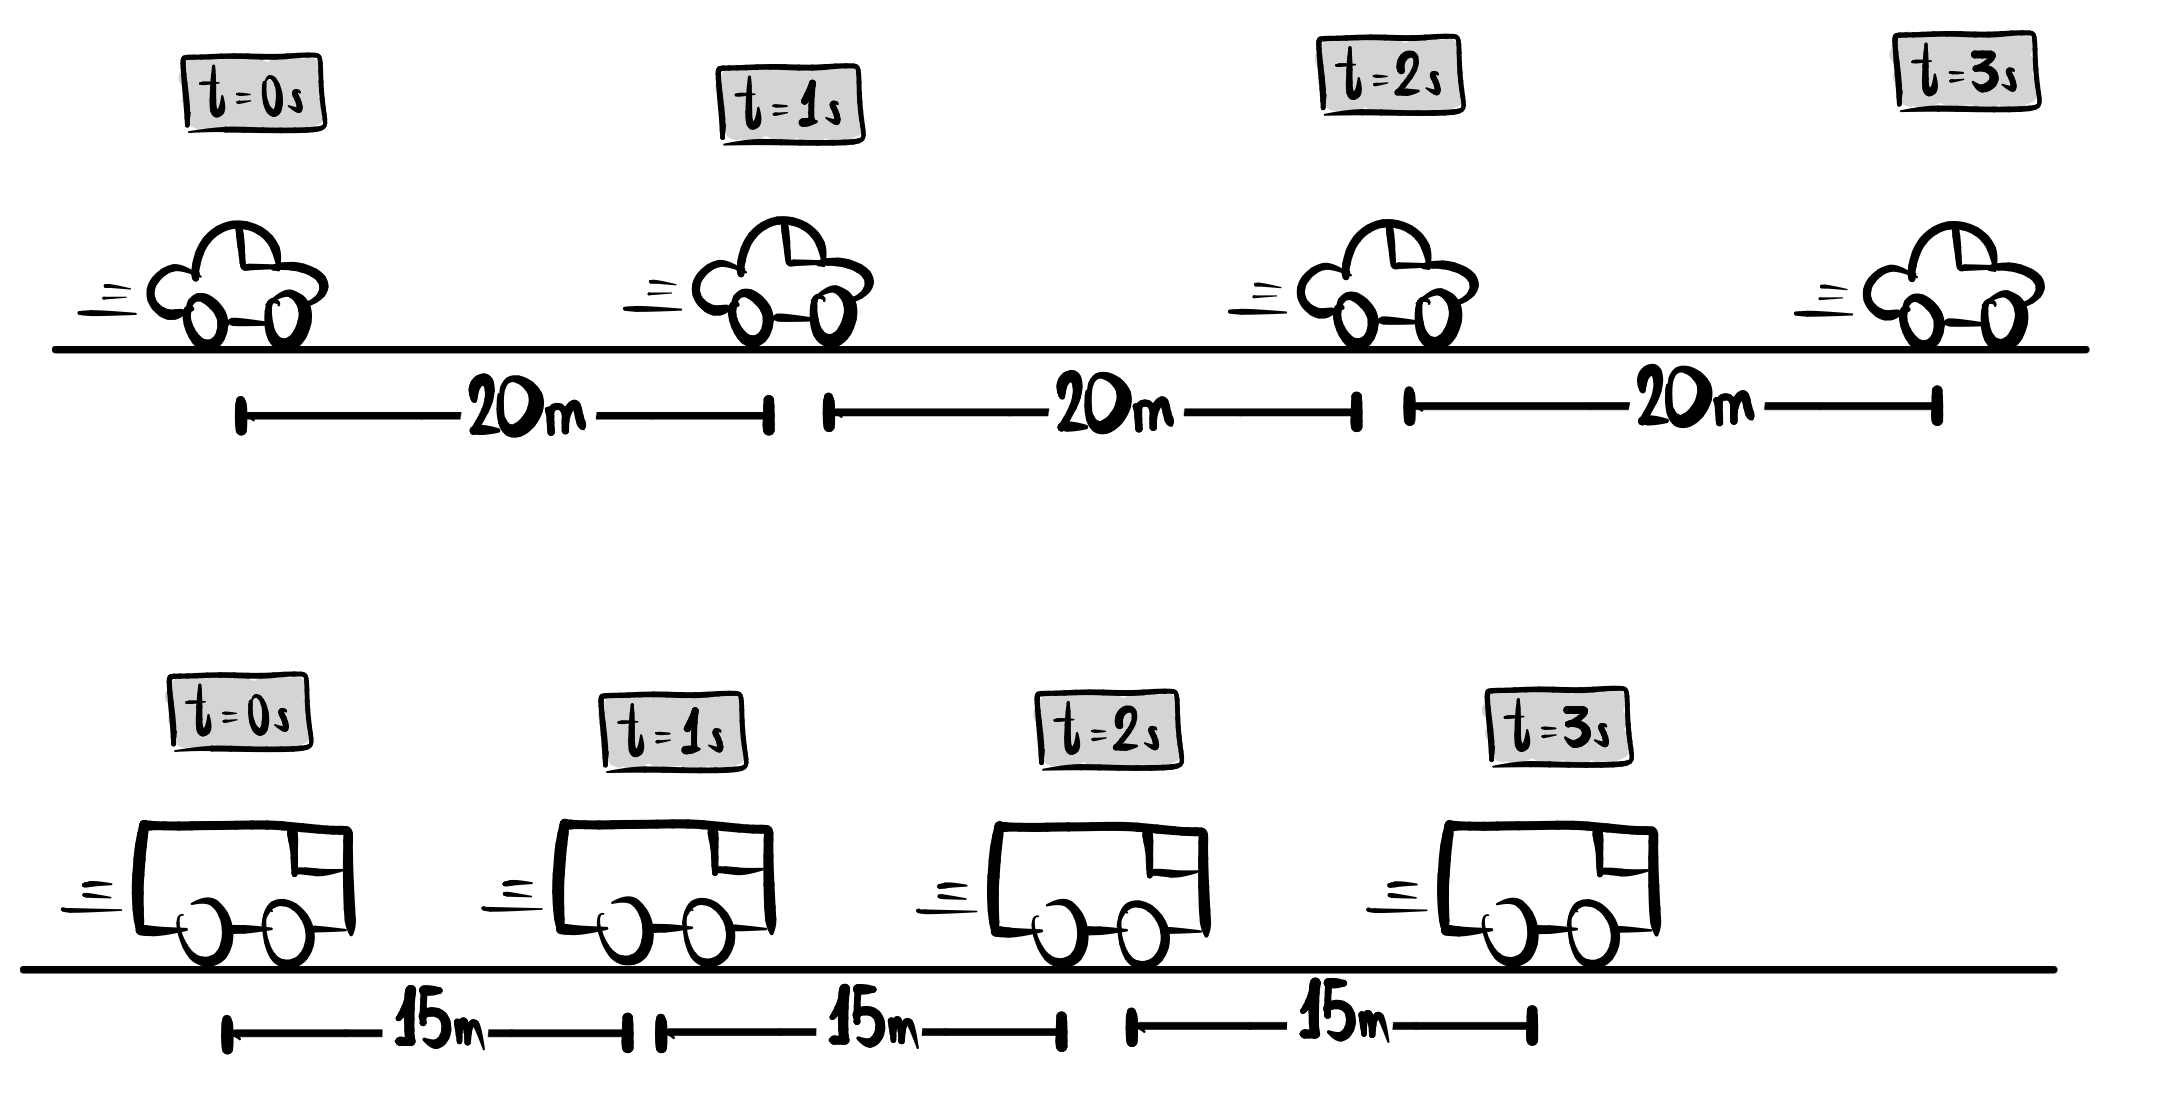
\includegraphics[scale=0.18]{imagensintro/carros.jpeg}};
      \end{scope}
    \end{tikzpicture}
    \caption{Comparando o movimento de dois objetos em um universo em que o conceito de velocidade é inexistente.}
    \label{intro04}
\end{figure}


Eu poderia começar lhe dizendo que existe um carro e um ônibus, os dois se movendo em uma mesma direção, porém o carro anda mais depressa que o ônibus. Isso estaria correto, porém um pouco incompleto. O quão mais depressa se move esse carro? 
% Poderíamos tentar observar qual dos dois teria mais \emph{tracinhos} atrás, mas isso dependerá do cuidado e esmero de quem fez as imagens para transmitir a rapidez de cada um com precisão.

Note que, para tentar dizer isso, eu começaria, em alguma medida, a enfrentar problemas parecidos com aquele da mesa do café da manhã, pela simples razão de limitação linguística --- não há um termo para medir o quão rápido algo se move na nossa linguagem, pelo menos até então. 

Eu poderia, então, lhe dizer que o carro anda cinco metros a mais que o ônibus em um mesmo intervalo de tempo, o que estaria correto, mas ainda deixaria espaço para imprecisão: você poderia pensar que o ônibus anda, a cada segundo, 80 metros, enquanto o carro andaria 85 metros. Quaisquer combinações de números em que um deles é cinco unidades maior do que o outro funcionariam e a informação que eu lhe transmiti, portanto, deixaria um grande espaço para ambiguidade. 

Talvez eu pudesse então logo lhe dizer o seguinte: \textit{existe um ônibus e um carro se movendo, em uma mesma direção e sentido, e enquanto o ônibus avança 15 metros, o carro avança 20 metros.} Pronto, agora não há espaço algum para ambiguidade: qualquer um conseguiria reconstruir, do zero, a Figura \ref{intro04} com base nessa informação. Quer dizer...alguém poderia, com base nessa informação, desenhar uma figura em que o carro avança 20 metros em 1 hora e o ônibus avança 15 metros durante essa mesma hora. Isso estaria coerente com a informação que fora transmitida, porém incoerente com a situação física real. 

Cansado de tentar explicar de forma sucinta a situação em questão, você simplesmente abandona tal missão e resolve descrever, \textit{ipsis litteris}, o que vê na figura: \textit{existe um ônibus e um carro se movendo na mesma direção e sentido, e enquanto o ônibus avança 15 metros durante o intervalo de tempo de 1 segundo, o carro avança 20 metros, neste mesmo intervalo de tempo de 1 segundo.}

Pronto, deu-se cabo de tal tarefa: não haverá cristão que discorde que tal frase transmite, na íntegra, toda a situação física da Figura \ref{intro04}. O que é verdade, porém foram necessárias algumas tentativas e, por fim, uma frase de três linhas para dar conta de tal tarefa.

Digamos, portanto, que, tal como nosso amigo Jairo o fez com a colher, resolvamos criar um novo conceito --- uma nova palavra --- para possibilitar facilitar e comunicar situações como as da Figura \ref{intro04}. Incumbido de tal missão, eis que o leitor, inspirado pelo espírito e feito de Jairo, sobe na cadeira, com o peito estufado, braço direito erguido e postura ereta, e grita aos que estão à sua volta:

\begin{center}
    \textit{Doravante, a razão entre a distância percorrida por um corpo e o intervalo de tempo no qual tal distância é percorrida será chamada de velocidade!}
\end{center}

Pronto: foi feito o batismo. Todos se emocionam e se arrepiam diante da grande honra que é viver tal momento em que uma nova grandeza física é criada. Em termos matemáticos, o que você fez foi dizer que, sendo $d$ a distância que um objeto percorre em um intervalo de tempo $\Delta t$, a sua velocidade, a qual denominaremos por $v$, é dada por

\begin{equation}
   \boxed{ v := \dfrac{d}{\Delta t}.}
   \label{00intro_eq_velocidade}
\end{equation}

E sim, é isso mesmo. Tal como foi necessário para Jairo criar um nome para um objeto a fim de ampliar sua capacidade de comunicação, o mesmo foi feito por nós: criamos um nome e uma equação matemática que \textbf{define} uma nova grandeza física, com o simples intuito de possibilitar que o estudo e a análise de situações como as da Figura \ref{intro04} sejam simplificados. 

Agora, analisando tal imagem e incumbido da nobre missão de transmitir toda a sua informação a alguém que não a viu, você poderia simplesmente dizer que:

\textit{Existe um ônibus e um carro se movendo, em uma mesma direção e sentido, sendo suas velocidades de $15$ m/s e $20$ m/s, respectivamente.}

Desde que esteja acordado e convencionado entre nós o que se trata o termo \textit{velocidade} --- tal e qual precisa estar acordado a que se refere o termo \textit{colher} --- tal frase transmite, com simplicidade, toda a informação física do contexto.



Algumas observações merecem ser feitas a respeito de tal definição:

\begin{itemize}
    \item [(i)] Simbologia

    O símbolo $:=$ que usamos talvez seja novo para o leitor. Confesso que acho seu uso desnecessário para o estudante de primeira viagem, mas fiz questão de usá-lo para deixar clara a natureza da equação física que apresentamos. Tal símbolo significa justamente que está ocorrendo uma definição, e é comum de ser utilizado assim que definimos (batizamos ou criamos, caso o leitor assim prefira) uma grandeza pela primeira vez. A fim de deixar nítida a diferença para o sinal de igualdade, perceba que as equações devem ser lidas como:

    \begin{align}
        v &= \sfrac{d}{\Delta t} \rightarrow v \text{ é igual a } d \text{ dividido por } \Delta t .\nonumber \\ 
        v &:= \sfrac{d}{\Delta t} \rightarrow v \text{ é definido como sendo } d \text{ dividido por } \Delta t  .\nonumber
    \end{align}

Uma vez que \textbf{definimos} $v$ como sendo $d$ dividido por $\Delta t$, é claro que $v$ passa ser \textbf{igual} a $d$ dividido por $\Delta t$, por definição. 

Ou seja, após o termo ter sido definido, podemos tranquilamente usar o símbolo de igualdade daí em diante, já que uma coisa equivale a outra. O símbolo $:=$, portanto, será usado exclusivamente na primeira vez em que estivermos definindo uma grandeza, e ele já deixará clara a natureza da equação física em questão: não se trata de uma equação experimental ou demonstrável, mas sim de uma definição.

    \item [(ii)] Significado

    De fato, o que estamos fazendo é realmente criar um novo termo: uma nova grandeza física. Isso não deveria lhe soar estranho, ou pelo menos não mais estranho do que o fato de que um dia alguém batizou o objeto da Figura \ref{intro01} como colher e começamos a nos referir a tal utensílio por tal nome, desde então. 
    
    Inventar verbos, criar nome para objetos ou para grandezas físicas faz parte da construção da linguagem, o que nos permite ampliar nossa capacidade, precisão e especificidade da comunicação. Seria muito difícil você expressar, em palavras, que gosta muito de alguém em uma sociedade na qual as palavras \textit{gostar} e \textit{amar} não existissem; da mesma forma que é difícil pedir a alguém uma colher se tal palavra não existe e também é um pouco complicado comparar a rapidez com que objetos se movem caso não exista o conceito de velocidade.
    
    É claro que alguém poderia, a seu bel prazer, criar uma nova grandeza física qualquer. Digamos que tal grandeza seja o número de janelas de uma casa dividido pelo número de portas, tudo isso elevado ao quadrado. Damos o nome a essa grandeza de Rudolph, representado pela letra $r$, e definido, portanto, por:

    $$ r : = \left( \dfrac{\text{número de janelas}}{\text{número de portas}} \right)^2.$$

    Ora, isso pode ser feito, mas qual seria a finalidade de inventarmos tal grandeza? Podemos, em teoria, inventar qualquer palavra ou qualquer grandeza física, mas, se isso não tiver uma finalidade ou serventia clara, certamente não será levado adiante. Acontece que criar uma grandeza física chamada \textit{velocidade} e defini-la conforme a Equação \eqref{00intro_eq_velocidade} parece fazer bastante sentido, uma vez que melhora nossa precisão na comunicação a respeito do movimento dos corpos, como vimos. 
    
    Note que o autor investiu um certo tempo, antes de apresentar tal fórmula, criando um contexto em que, ao final, ficasse claro como que a invenção de tal conceito resolveria alguns problemas de comunicação, eliminaria ambiguidades e possibilitaria que fosse possível transmitir informações a respeito de movimento de corpos com muito mais fluidez. Dito isso, parece fazer sentido criar tal conceito, tal como parecia fazer sentido criar um nome para o talher da Figura \ref{intro03}, fosse ele colher ou qualquer outro. Perceba que o nome da grandeza $v$ ser velocidade é pouco relevante --- caso ela se chamasse qualquer outra coisa ou fosse representada por qualquer outra letra, não teria muito problema. O que é relevante, de fato, é a sua definição matemática: ela representa a razão entre a distância percorrida e o tempo, e é isso, essencialmente, que a define. Do mesmo modo, se o nome do talher da Figura \ref{intro03} fosse, digamos, velocidade, não teria problema: temos um nome associado ao objeto, e isso é tudo que precisamos para estabelecer a comunicação.

    Note que, na grandeza Rudolph, nada disso se aplica: não parece ter sentido, serventia ou utilidade alguma em criar tal grandeza. Ela não facilita a comunicação de nada, até porque o número de janelas de uma casa pode ser importante, o número de portas também, mas ninguém está interessado em saber quanto vale a razão entre essas coisas elevado ao quadrado.

    Dito isso, ao definir qualquer grandeza, é importante que o leitor sempre se atente ao motivo pelo qual aquilo está sendo feito. Há algum sentido e razão em se criar um novo conceito, e é importante compreendê-lo para que o leitor entenda com profundidade o significado de tal equação, tal como fizemos, em parte, para criar o conceito de velocidade.

    

    

    \item [(iii)] Operacional

    Com tudo que construímos até aqui, parece que a única vantagem em se criar uma nova grandeza física, como a velocidade, é linguística: temos agora uma nova palavra, ou melhor, um novo conceito, para poder expressar algo que vemos no mundo. Isso é, em essência, o que Jairo fez ao criar a palavra colher.

    Contudo, esse não é o principal motivo de fazermos isso na Física. A definição de novas grandezas tem um caráter, acima de tudo, operacional. Como veremos, ao desdobrar os estudos da Física, em diversos contextos a rapidez com que um corpo se move ao longo do tempo --- a velocidade --- é um conceito que irá aparecer repetidas vezes, de modo que uma série de equações assumirão um caráter mais simples em termos dessa grandeza. Enuncio algumas delas abaixo, apenas para que o leitor tenha um gosto a respeito da importância de se criar o conceito de velocidade $v$:

    %$$ E_c = \dfrac{1}{2}mv^2 \text{  ;  } a_c = \dfrac{v^2}{R} \text{  ;  } F_M = Bqv \sin \theta \text{  ;  } \gamma = \dfrac{1}{\sqrt{1-\sfrac{v^2}{c^2}}}.$$

\[
\underbrace{E_c = \frac{1}{2}mv^2}_{\text{Energia cinética}} \quad ; \quad
\underbrace{a_c = \frac{v^2}{R}}_{\text{Aceleração centrípeta}} \quad ; \quad 
\underbrace{F_M = Bqv\sin\theta}_{\text{Força magnética}} \quad ; \quad
\underbrace{\gamma = \frac{1}{\sqrt{1 - \frac{v^2}{c^2}}}}_{\text{Fator de Lorentz}}
\]


Todas essas equações expressam grandezas físicas em termos de outras grandezas, sendo uma delas a velocidade $v$. Desse modo, ter criado o conceito de velocidade definido da forma como foi feito na Equação \eqref{00intro_eq_velocidade} se mostrará algo extremamente relevante: construiremos outras grandezas, equações e teorias em cima de tal noção, o que nos trará uma vantagem operacional ao longo dos cálculos.

\end{itemize}



Por fim, que fique claro para o leitor: as equações desse tipo --- as definições --- são expressões matemáticas que não descrevem a natureza, mas sim criam o vocabulário com o qual a natureza será descrita. O que estamos fazendo aqui, como a poetisa escreveu nos versos, é estabelecer o acordo para que consigamos fazer uma boa comunicação. Este é o primeiro tipo de equação que o leitor precisa conhecer. Note que, ao definirmos o conceito de velocidade, não estamos dizendo absolutamente nada a respeito de como a natureza funciona. Estamos apenas estabelecendo a linguagem que iremos utilizar para, aí sim, estudar a natureza e entender como ela funciona. \footnote{Como o objetivo desse tipo de equação é criar o vocabulário para construir, em cima dele, o conhecimento teórico, o leitor há de notar que, ao iniciar o estudo de uma nova parte da Física, quase sempre ele começará por meio de algumas definições. Ao começar o estudo de movimento precisamos criar o conceito de velocidade, de aceleração...ao começar o estudo de circuitos elétricos precisamos criar o conceito de corrente elétrica --- isto é, definir esta nova grandeza em termos de outras --- ao começar o estudo de óptica precisaremos definir o que é o índice de refração, e por aí vai. }




\subsection{Equações Experimentais}

O segundo tipo de equação que podemos encontrar na Física é o das equações experimentais. Esse tipo de equação não é uma invenção humana, logo, sua razão de ser não é estabelecer o vocabulário que será usado para o estudo. Equações desse tipo expressam, em linguagem matemática, como a natureza se comporta em certo contexto ou fenômeno. Ou seja, faz-se um experimento, digamos, como o da Figura \ref{intro02}, e sintetiza-se, matematicamente, o resultado de tal experimento por meio de um equação, como a Equação \eqref{00intro_eq_quedalivre}. Perceba que nós não inventamos tal equação\footnote{Pode haver alguma ambiguidade entre equações experimentais e equações demonstráveis, que serão as próximas a serem estudadas. Sobre isso, sugerimos ao leitor, após concluir a introdução e avançar bastante ao longo do texto para ganhar um pouco mais de maturidade, ler o \autoref{apendice-eqs-exp-vs-dem}.} --- e ela tampouco se propõe a definir ou criar algum conceito. Ela simplesmente traduz, em linguagem matemática, o que foi observado no experimento.

Para citar um outro exemplo, observe a Figura \ref{intro07}, que mostra duas cargas elétricas positivas, de cargas $Q_1$ e $Q_2$, separadas por uma distância $r$.

\begin{figure}[h]
    \centering
    \begin{tikzpicture}
      \begin{scope}[blend mode=multiply]
        \node {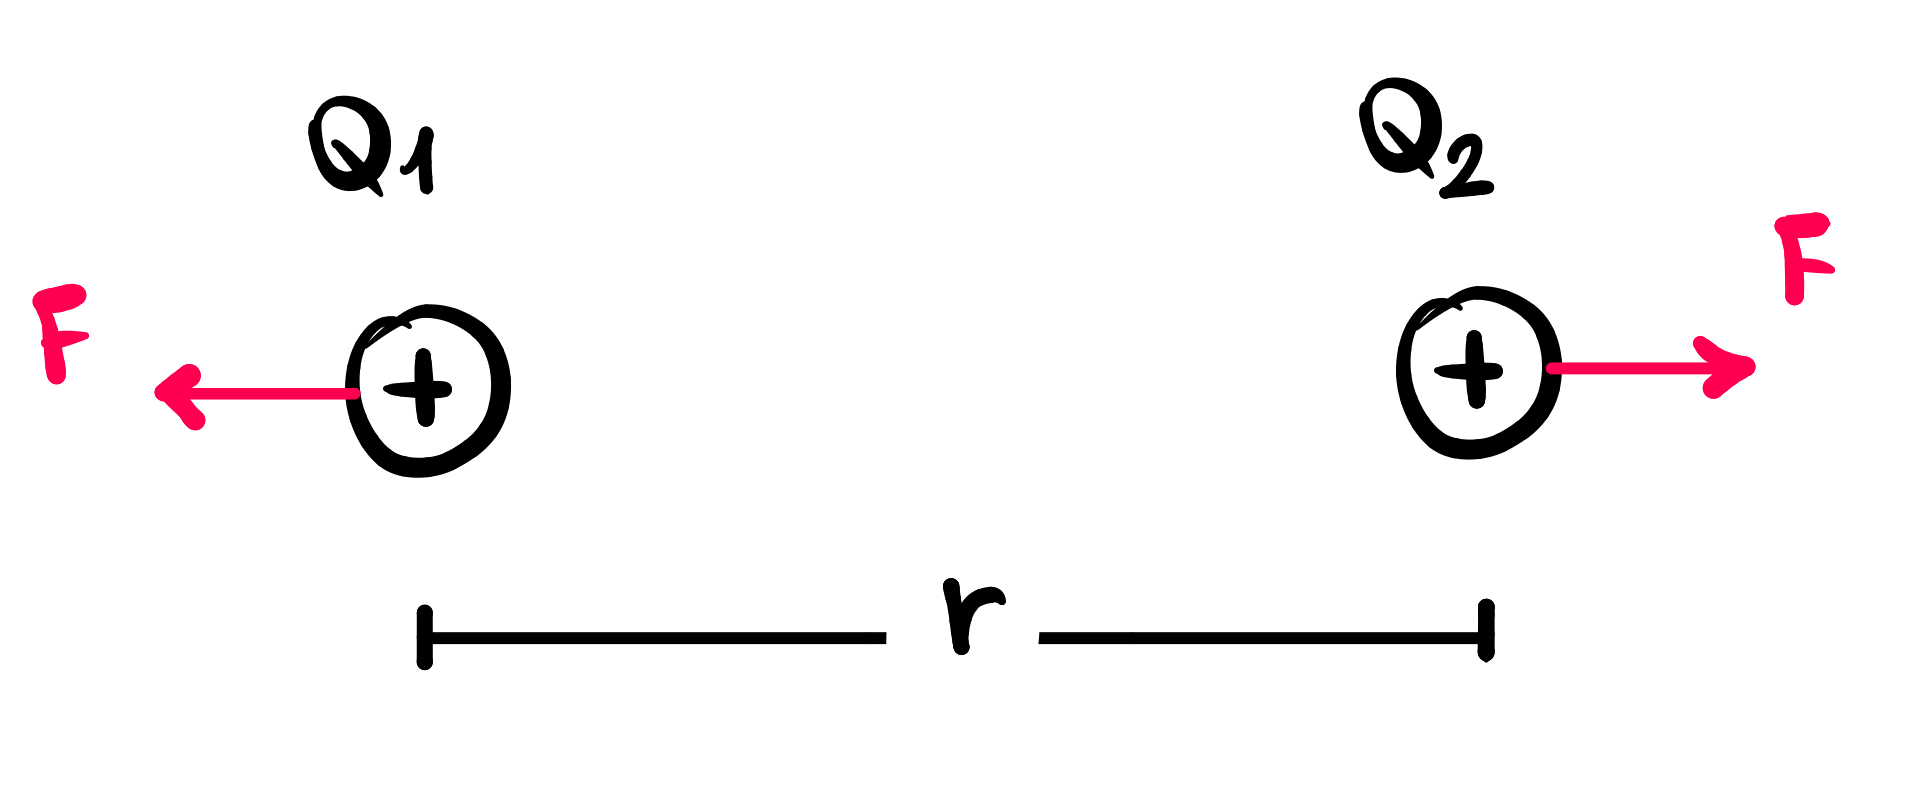
\includegraphics[scale=0.12]{imagensintro/coulomb.jpeg}};
      \end{scope}
    \end{tikzpicture}
    \caption{A força eletrostática entre duas cargas elétricas $Q_1$ e $Q_2$.}
    \label{intro07}
\end{figure}


Já era conhecido, desde o século XVII, que corpos eletrizados poderiam se atrair ou se repelir, porém ninguém sabia exatamente como poderíamos computar tal força. Em 1785, um físico francês chamado Charles-Augustin de Coulomb introduziu um aparato, chamado balança de torção, que o possibilitou fazer alguns experimentos para identificar como se dava tal força (explicaremos em mais detalhes o que é isso e como o experimento foi feito no momento adequado).

Ao fazer vários experimentos, com diferentes valores de cargas elétricas $Q$ e diferentes valores de distância $r$ entre as cargas, o aparato de Coulomb possibilitava medir a força elétrica entre as cargas da Figura \ref{intro07}. Após várias medições, foram percebidos dois fatos experimentais fundamentais:

\begin{itemize}
    \item A força é proporcional ao produto das cargas $Q_1 \cdot Q_2.$
    \item A força diminui com o quadrado da distância entre as cargas, ou seja, é proporcional a $\dfrac{1}{r^2}.$
\end{itemize}


Nada disso foi definido ou deduzido. Tudo isso foi inferido a partir de dados experimentais. Com o tempo, foi possível construir uma equação matemática que sintetizasse os dados do experimento, que é a equação conhecida como Lei de Coulomb, dada por

\begin{equation}
    F = k \dfrac{Q_1Q_2}{r^2},
    \label{00intro_eq_coulomb}
\end{equation}
em que $k$ é uma constante que é obtida pelos experimentos. Note que a Equação \eqref{00intro_eq_coulomb} sintetiza os dois fatos que foram observados anteriormente: a força é proporcional ao produto das cargas e inversamente proporcional ao quadrado da distância. Trata-se apenas de se transmitir, matematicamente, a informação a respeito de como a natureza funciona, informação esta que foi obtida por meio da realização de um experimento.

Observe que a Lei de Coulomb não é uma definição: ela não define ou explica o que é uma carga elétrica ou o que é uma força. Ao mesmo tempo, tal lei tampouco explica porque a força tem essa forma, ou como essa força é transmitida de uma carga para outra. Ela apenas afirma que é assim que a força se comporta, como foi observado no experimento.

A essa altura o leitor pode se sentir um pouco insatisfeito, talvez por ter enxergado uma aparente limitação nesse tipo de fórmula, o que pode tê-lo levado a questionamentos como

\begin{center}
    \textit{Temos só que aceitar que a fórmula é essa? De onde vem essa força, e por que ela funciona assim?}
\end{center}

Essa sensação é natural, mas é preciso deixar claro desde já: essa limitação não é um defeito da equação experimental. Ela é, na verdade, sua \textbf{característica essencial.}

Uma equação experimental não pretende explicar por que a natureza funciona de determinado modo.
Ela descreve como a natureza se comporta, dentro de um certo contexto observável.
O experimento nos permite medir, comparar, identificar regularidades e, a partir disso, sintetizar esse comportamento em linguagem matemática. É exatamente isso que a equação expressa: um retrato fiel do \textit{como.}

Por que ela funciona exatamente assim é algo que podemos responder com a criação de alguma teoria mais ampla que tente entender o motivo de tal funcionamento, ou, talvez, nunca conseguiremos responder. Em última instância, sempre chegaremos a alguma pergunta que não conseguiremos responder, que talvez se torne mais filosófica do que física.

%Para exemplificar isso, vamos voltar ao experimento de abandonar a pedra e analisar seu movimento, descrito na Figura \ref{intro02}. O experimento nos permite entender como se dá o movimento da pedra: em intervalos de tempos sucessivos as distâncias percorridas estão na proporção dos números ímpares. Isso pode ser transmitido dessa forma, ou em linguagem matemática, como a Equação \eqref{00intro_eq_quedalivre} se propõe a fazer. Note que, até aqui, não sabemos exatamente porque a pedra cai. Sabemos só que ela cai --- e sabemos que esse movimento evolui ao longo tempo de um jeito específico. Alguém poderia até perguntar: \textit{mas por quê a pedra cai?}.

Para tornar isso concreto, voltemos ao experimento simples de abandonar uma pedra e observar seu movimento, ilustrado na Figura~\ref{intro02}. O experimento nos mostra como a pedra se move: em intervalos de tempo sucessivos, as distâncias percorridas seguem a proporção dos números ímpares. Esse padrão pode ser descrito verbalmente ou condensado em linguagem matemática, como faz a Equação~\eqref{00intro_eq_quedalivre}.

Até aqui, tudo o que sabemos é como a pedra cai. Sabemos que ela cai. Sabemos que seu movimento evolui no tempo de uma forma específica e regular. Mas nada disso responde à pergunta: por que a pedra cai? E é importante perceber que o experimento, por si só, não pode responder a essa pergunta. Esse é precisamente o ponto.

A equação experimental não nasce para explicar causas profundas, mas para organizar o comportamento observado. Ela é uma síntese matemática do que pode ser medido, não uma explicação sobre por que as coisas funcionam como funcionam.

%Perceba que tal experimento não nos permite responder essa pergunta --- e essa é grande característica da equação experimental, como eu estava dizendo. Ela traduz uma síntese de \textit{como} a natureza funciona, que é o que o experimento nos permite medir e identificar, e não do \textit{por que} ela funciona dessa forma. 

É claro que alguém pode, posteriormente, propor uma teoria que tente responder a esse “porquê”. Foi exatamente isso que Newton fez ao formular sua teoria da gravitação. Agora, com essa nova estrutura conceitual, somos capazes de dizer: a pedra cai por causa da gravidade. Mas isso apenas desloca a pergunta. \textit{Por que a gravidade existe? Como ela se propaga? } 

O próprio Newton não saberia responder essas duas últimas perguntas. E, como disse, se formos avançando, provavelmente chegaremos em alguma pergunta que será mais filosófica do que física, e seremos obrigados a parar em algum momento. Em algum momento, talvez, teremos que ficar satisfeitos em entender como a natureza funciona, sem saber exatamente o motivo de ser assim.

É isso. Uma equação experimental é uma síntese matemática de \textit{como} a natureza funciona em um certo contexto. É uma equação que nasce do experimento, não da dedução lógica nem da definição conceitual. Ela surge quando medições revelam regularidades, quando padrões numéricos se repetem e é possível encontrar uma relação matemática simples capaz de condensar os dados.








\subsection{Equações Demonstráveis}

Vamos ao terceiro e último tipo possível de equação que podemos encontrar na Física: equações demonstráveis. Elas não são definições --- não servem para criar vocabulário e estabelecer novos conceitos. Ao mesmo tempo, elas também não são meramente uma expressão do resultado de algum experimento físico. O que elas são, então?

Para responder a essa pergunta, carece voltarmos ao século III a.C. para considerar a estruturação da lógica feita por Aristóteles. O filósofo grego criou o silogismo, que é um raciocínio dedutivo que parte de algumas premissas (afirmações iniciais) para chegar a uma \textbf{conclusão lógica.} O exemplo mais simples e conhecido possivelmente é: 

\begin{quote}
    P1: Todo homem é mortal.\\
    P2: Sócrates é homem.\\
    C: Logo, Sócrates é mortal.
\end{quote}


As duas primeiras frases são as nossas \textit{premissas:} afirmações que aceitamos como verdade. A terceira frase é nossa conclusão: uma consequência lógica e inevitável de termos aceitado como verdadeiras as duas premissas iniciais.

Note que é possível que se discorde das premissas. Alguém poderia questionar se todo homem é mesmo mortal, talvez acreditando que a ciência moderna desenvolverá tecnologias que permitam com que se viva para sempre. Também poderia haver um questionamento sobre Sócrates ser mesmo homem. Quem foi este ser? Será que ele existiu de fato? E, se o fez, quem me garante que ele não era um cachorro, mas sim um homem?

Ora, questionamentos como estes são até válidos, mas note que, se assumirmos as premissas como verdadeiras, a conclusão é inevitável, é absolutamente inquestionável: um estatuto estabelecido --- cuja veracidade depende, naturalmente, da veracidade das premissas. Se a conclusão não for compatível com a realidade --- isto é, se averiguarmos que o tal Sócrates não é mortal --- o erro não estaria na conclusão --- esta é logicamente irrefutável --- e sim nas premissas. Provavelmente teríamos errado ao assumir que todo homem é mortal, ou que Sócrates fosse homem...

Talvez o leitor prefira uma linguagem mais visual para compreender tal raciocínio, o que pode ser feito usando a teoria de conjuntos, como mostra a Figura \ref{intro06}. O que estamos dizendo é que existe um conjunto $M$ de todos os seres que são mortais. A primeira premissa diz que o conjunto $H$ de todos os homens faz parte do tal grupo $M,$ dos mortais. A segunda premissa diz que Sócrates faz parte do grupo $H$, dos homens, de onde devemos concluir, logicamente, que Sócrates, portanto, faz parte do grupo $M$ dos mortais, uma vez que ele contém o grupo dos homens.


\begin{figure}[h]
    \centering
    \begin{tikzpicture}
      \begin{scope}[blend mode=multiply]
        \node {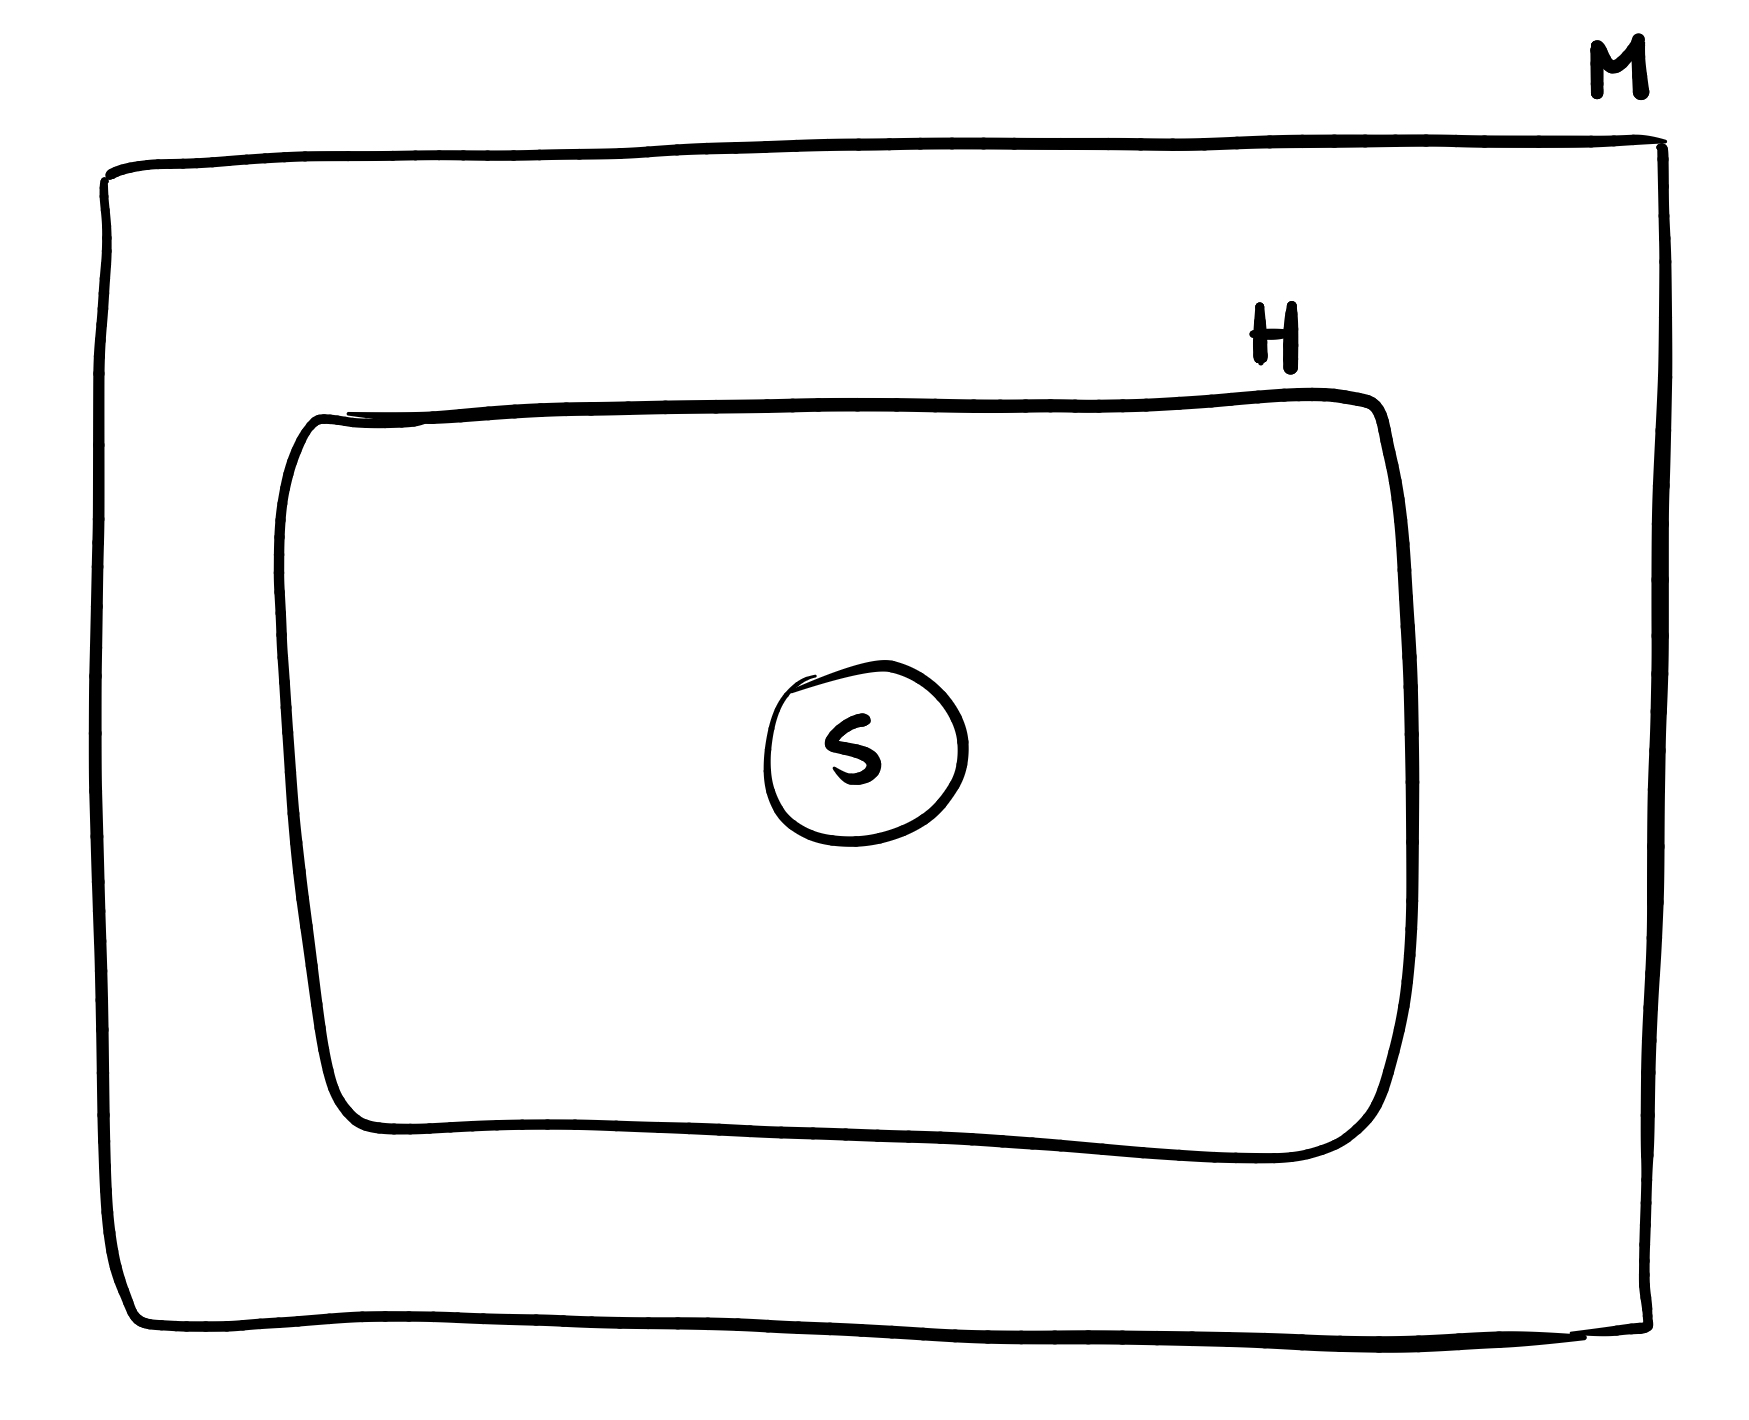
\includegraphics[scale=0.10]{imagensintro/socrates.jpeg}};
      \end{scope}
    \end{tikzpicture}
    \caption{Existe o grupo dos mortais, e a premissa P1 afirma que os homens fazem parte desse grupo. A premissa P2 afirma que Sócrates faz parte do grupo dos homens, logo, concluímos que Sócrates também faz parte do grupo dos mortais.}
    \label{intro06}
\end{figure}



Nessa analogia, as premissas seriam os princípios que fundamentam a nossa teoria física, e a conclusão seria uma equação matemática derivada de tais premissas, isto é, uma equação matemática que expressa uma conclusão lógica e irrefutável uma vez que se assume os princípios da teoria como verdadeiros. 

Poderíamos, por exemplo, criar uma teoria a respeito de como a luz se propaga. Tal teoria poderia enunciar, como princípio fundamental, que a luz se move de modo a sempre minimizar o tempo de percurso (o que de fato ocorre, e é conhecido como Princípio de Fermat, como veremos mais adiante). Além disso, poderíamos definir uma nova grandeza, o índice de refração $n$, de modo que seria possível construirmos o silogismo:

\begin{quote}
    P1: A luz se move de modo a sempre percorrer o trajeto que minimiza o tempo de percurso.\\
    P2: O índice de refração $n$ de um meio é definido como sendo $n := \sfrac{c}{v},$ em que $v$ é a velocidade da luz no meio e $c$ é a velocidade da luz no vácuo.\\
    C: Logo, ao mudar de meio, o comportamento da luz é governado pela equação matemática
    
    $$n_1 \sin \theta_1 = n_2 \sin \theta_2. $$
\end{quote}

Sim, eu sei: a conclusão não parece nada óbvia. Concluir que Sócrates era mortal foi muito mais fácil, mas acredite em mim: aqui estamos fazendo a mesma coisa. O fato de que a equação que governa a refração da luz --- ilustrada na Figura \ref{intro05} --- é aquela não ficou nada claro. Isso porque são necessários alguns passos intermediários de desenvolvimento matemático, o que será feito em momento oportuno. 


\begin{figure}[h]
    \centering
    \begin{tikzpicture}
      \begin{scope}[blend mode=multiply]
        \node {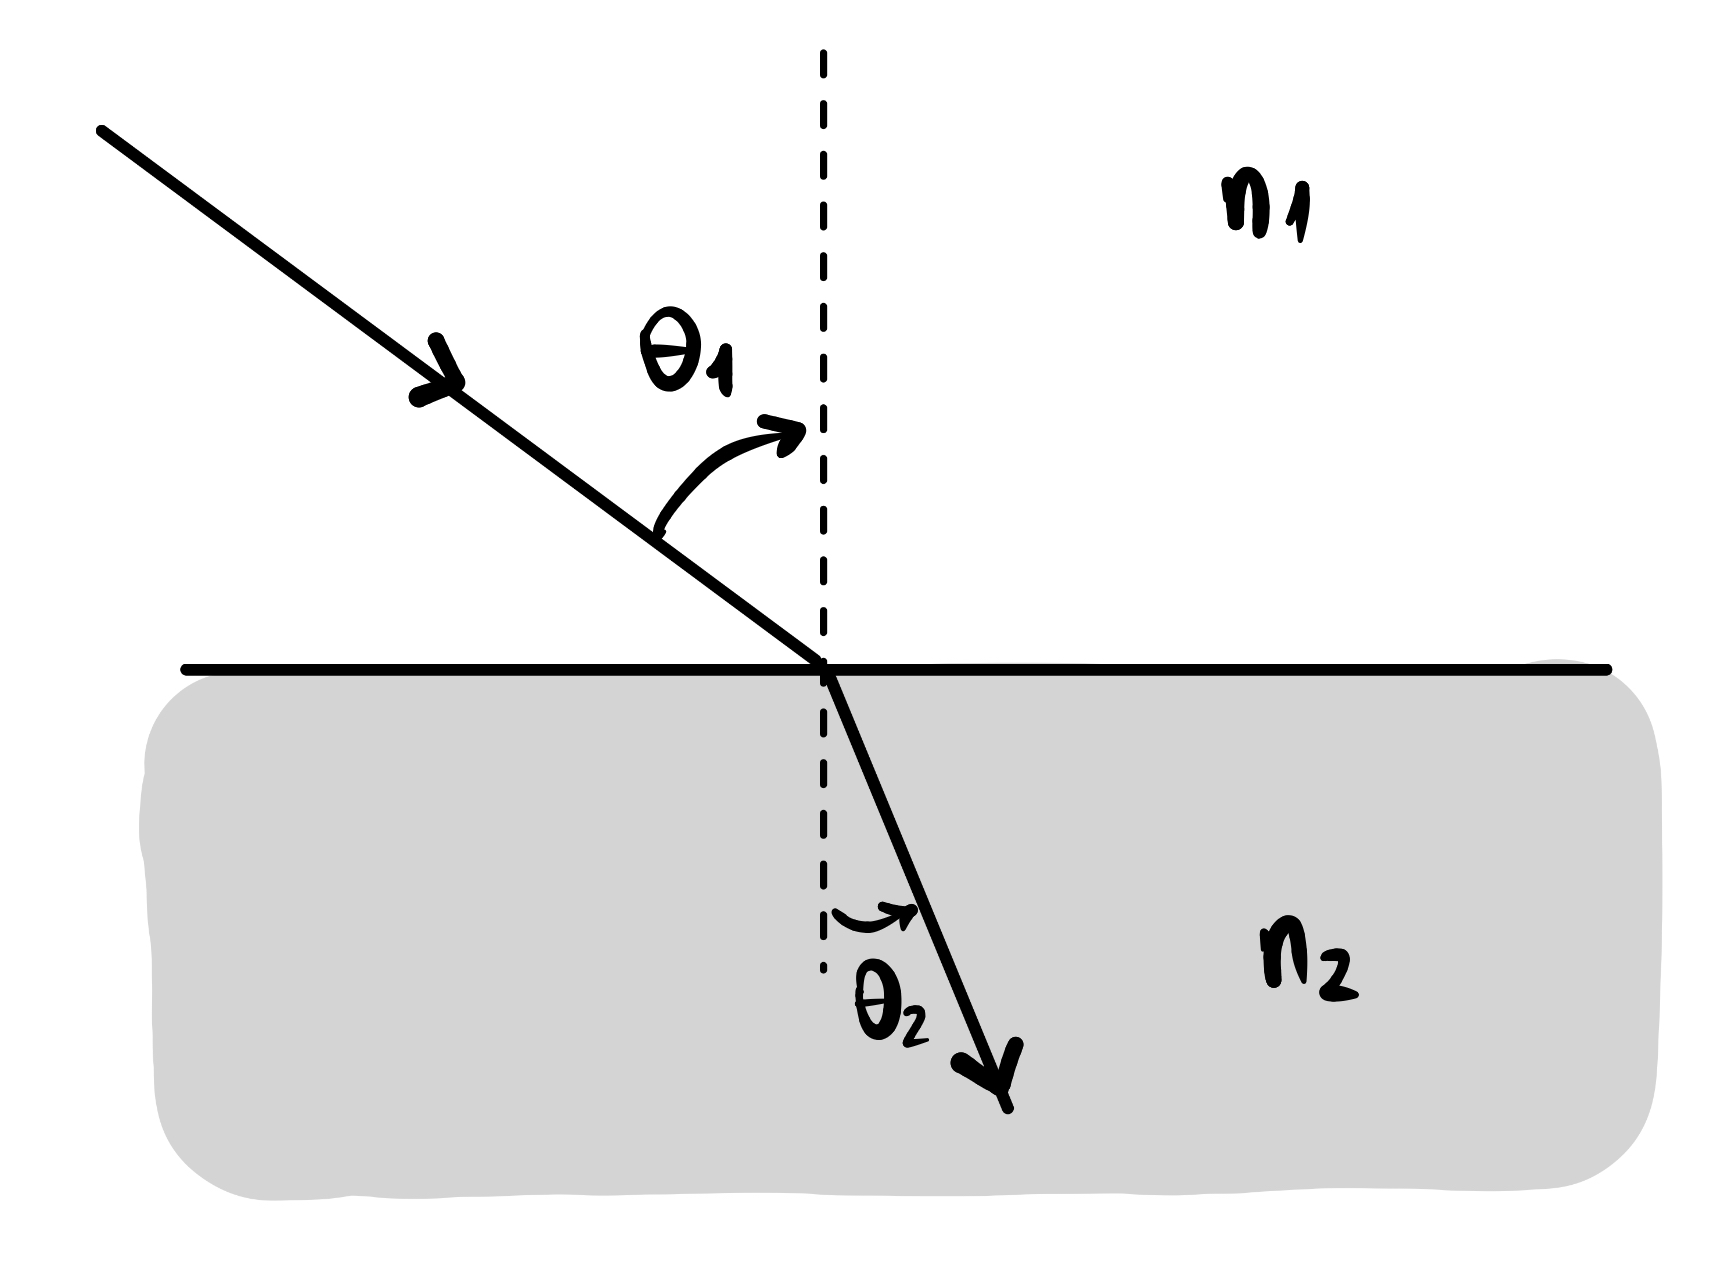
\includegraphics[scale=0.10]{imagensintro/refracao.jpeg}};
      \end{scope}
    \end{tikzpicture}
    \caption{Refração da luz.}
    \label{intro05}
\end{figure}

Contudo, para além da diferença no nível de dificuldade, o que foi feito acima é exatamente igual ao silogismo sobre a mortalidade de Sócrates. Assim, eis o nosso terceiro tipo de equação física: consequências lógicas e inevitáveis de termos assumido como verdadeiros os princípios da nossa teoria.

Tais equações, portanto, podem ser demonstradas, isto é, explicadas e construídas do zero com base nos pressupostos da teoria. Este é um tipo bem particular de equação, haja vista que as definições podem, no máximo, ser bem motivadas, mas elas são criações --- invenções humanas para estabelecer o vocabulário da teoria. Já as equações experimentais não têm nenhum tipo de margem para intervenção humana: elas são, letra por letra, governadas pelo experimento --- elas não dizem nada mais nada menos do que o experimento revelou. Já este terceiro tipo de equação, as demonstráveis, serão as que exigirão mais criatividade e arcabouço matemático, uma vez que elas são ``informações ocultas'' da teoria: elas estão ali, e dizem algo a respeito de como a natureza funciona, mas precisam ser encontradas e desvendadas, respeitando, naturalmente, as leis da lógica. Elas não estão explícitas, como as premissas, mas sim implícitas, e é preciso um olhar atento e refinado para conseguir extrair as conclusões que nos levarão a tais equações, que, como toda equação, apenas contém uma informação --- em linguagem matemática --- a respeito de como a natureza funciona.

Vejamos, a título de ilustração, algumas outras equações que são desse mesmo tipo.




\subsubsection{Período do Pêndulo Simples}

No século XVII, Galileu havia observado o \textit{isocronismo dos pêndulos de comprimentos idênticos,} ou seja, que pêndulos de mesmo comprimento sempre possuem o mesmo período de oscilação,\footnote{Do grego, \textit{iso = igualdade} e \textit{chronos = tempo}} independentemente da massa do objeto que está amarrada em sua extremidade. Ou seja, os três pêndulos da Figura \ref{intro06pend}, por terem o mesmo comprimento, terão exatamente o mesmo período de oscilação (tempo para que a massa vá de um extremo ao outro, retornando ao ponto inicial), independentemente dos valores das massas amarradas na sua extremidade.



\begin{figure}[h]
    \centering
    \begin{tikzpicture}
      \begin{scope}[blend mode=multiply]
        \node {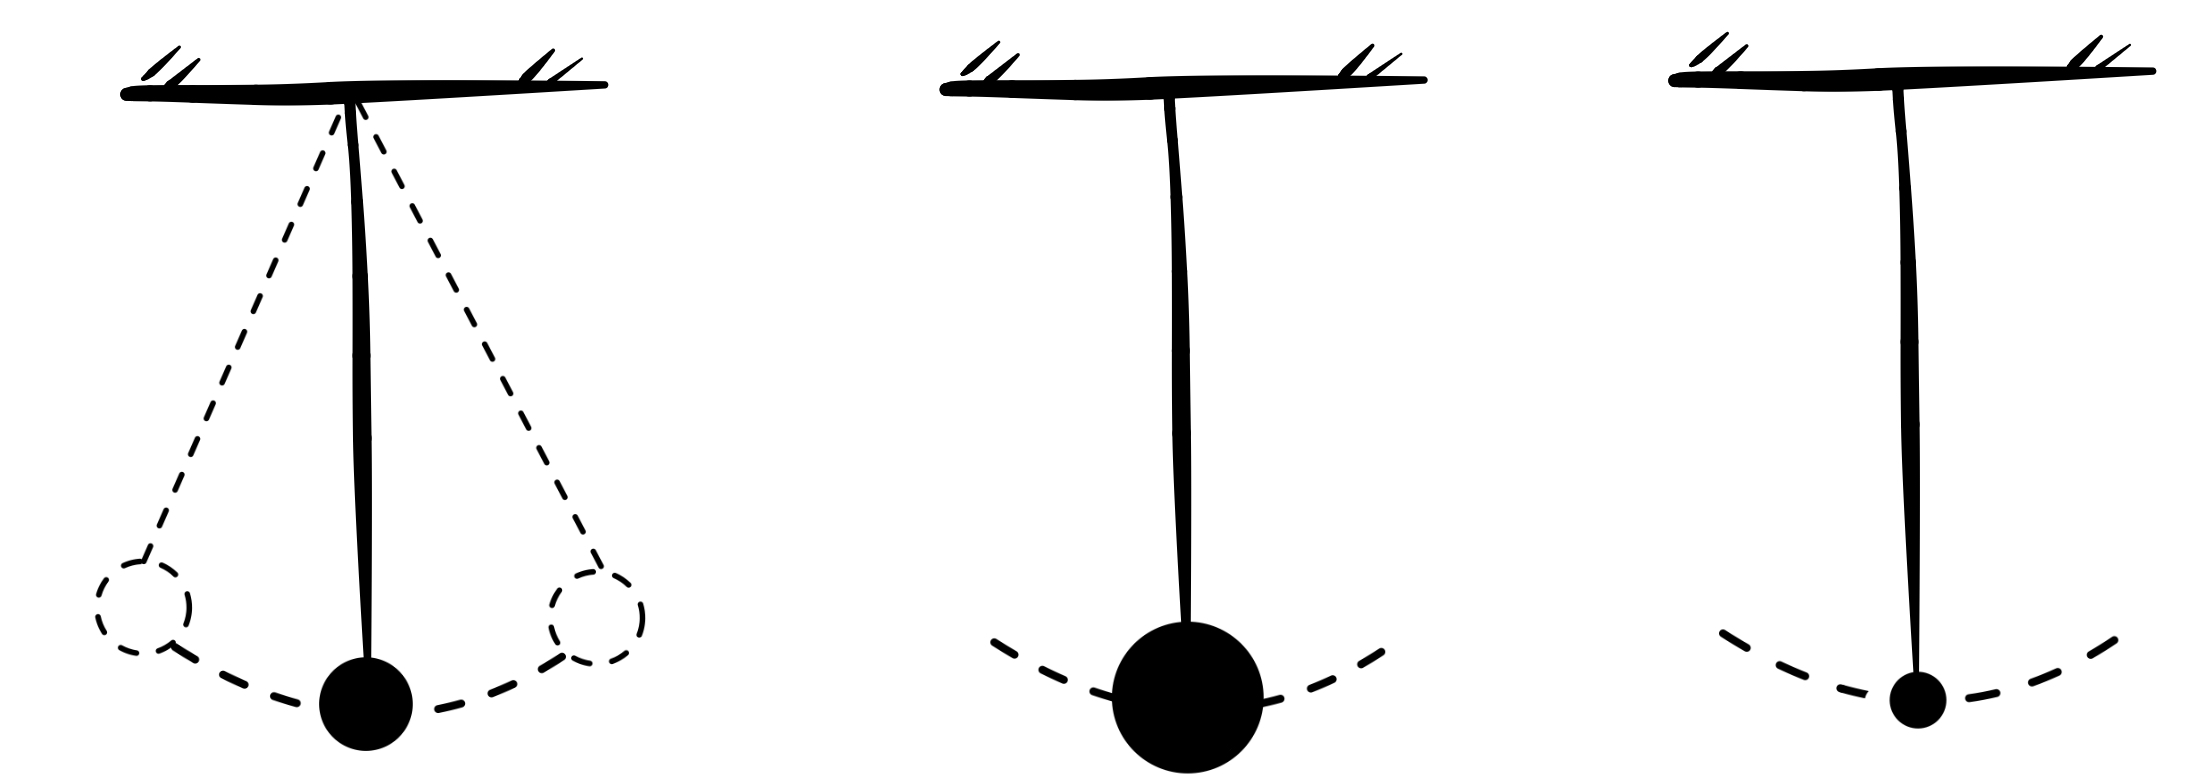
\includegraphics[scale=0.10]{imagensintro/pendulo.jpeg}};
      \end{scope}
    \end{tikzpicture}
    \caption{Oscilação do pêndulo simples.}
    \label{intro06pend}
\end{figure}


Que pêndulos de mesmo comprimento $l$ possuem o mesmo período de oscilação $T$, portanto, é um fato experimental. Contudo, podemos demonstrar, usando a teoria da dinâmica newtoniana e algumas premissas sobre o movimento oscilatório (não faremos isso neste momento) que o período de oscilação $T$ do pêndulo simples é dado por

\begin{equation}
    T = 2\pi \sqrt{\dfrac{l}{g}},
    \label{00intro_eq_pendulo}
\end{equation}
em que $g$ é a aceleração da gravidade e $l$ é o comprimento do pêndulo. Tal equação não é uma definição --- não estamos definindo nenhuma grandeza nova aqui --- e tampouco exprime simplesmente o resultado de algum experimento. Note que a equação, naturalmente, está de acordo com o experimento: o período depende do comprimento $l$ do fio, mas não da massa $m$ amarrada na sua extremidade, de modo que pêndulos de mesmo comprimento $l$ terão o mesmo período de oscilação qualquer que seja a massa amarrada em suas extremidades.

A Equação \eqref{00intro_eq_pendulo}, portanto, vai além: ela nos diz exatamente como pode-se calcular com precisão o período de um pêndulo simples qualquer\footnote{Para pequenas oscilações, como veremos em detalhes no estudo do volume II dessa coleção.}. Ela é uma consequência lógica dos princípios da teoria, expressando uma faceta a respeito de como a natureza funciona, no caso, como certos tipos de objetos oscilam sob a ação da gravidade. 

Tal equação, portanto, é uma conclusão (no sentido da lógica aristotélica): ela é uma consequência lógica dos pressupostos da teoria e, naturalmente, nos diz algo a respeito do funcionamento do universo. O fato do experimento concordar com o que tal conclusão diz é um bom indicativo de que as premissas da teoria devem estar corretas.

Quais são as premissas e como é o desenvolvimento lógico para nos permitir tirar a conclusão e desaguar na Equação \eqref{00intro_eq_pendulo} é algo que será feito em um momento futuro. Por hora, é importante que o leitor entenda apenas a diferença entre esse novo tipo de equação e os dois tipos anteriores.




\subsubsection{Equação Fundamental da Ondulatória}

Este é um exemplo de natureza mais simples, de modo que faremos seu desenvolvimento completo, para tentar trazer mais clareza ao leitor sobre esse tipo de equação.

Dada uma onda de \textit{comprimento de onda} $\lambda$ (isso é uma definição: criação de vocabulário para nos permitir construir a teoria), frequência $f$ (também uma definição) e velocidade de propagação $v,$ como mostra a Figura \ref{introonda}, essas três grandezas se relacionam por meio da Equação Fundamental da Ondulatória, que estabelece que

\begin{equation}
    v = \lambda f.
    \label{00intro_eq_vlambdaf}
\end{equation}

\begin{figure}[h]
    \centering
    \begin{tikzpicture}
      \begin{scope}[blend mode=multiply]
        \node {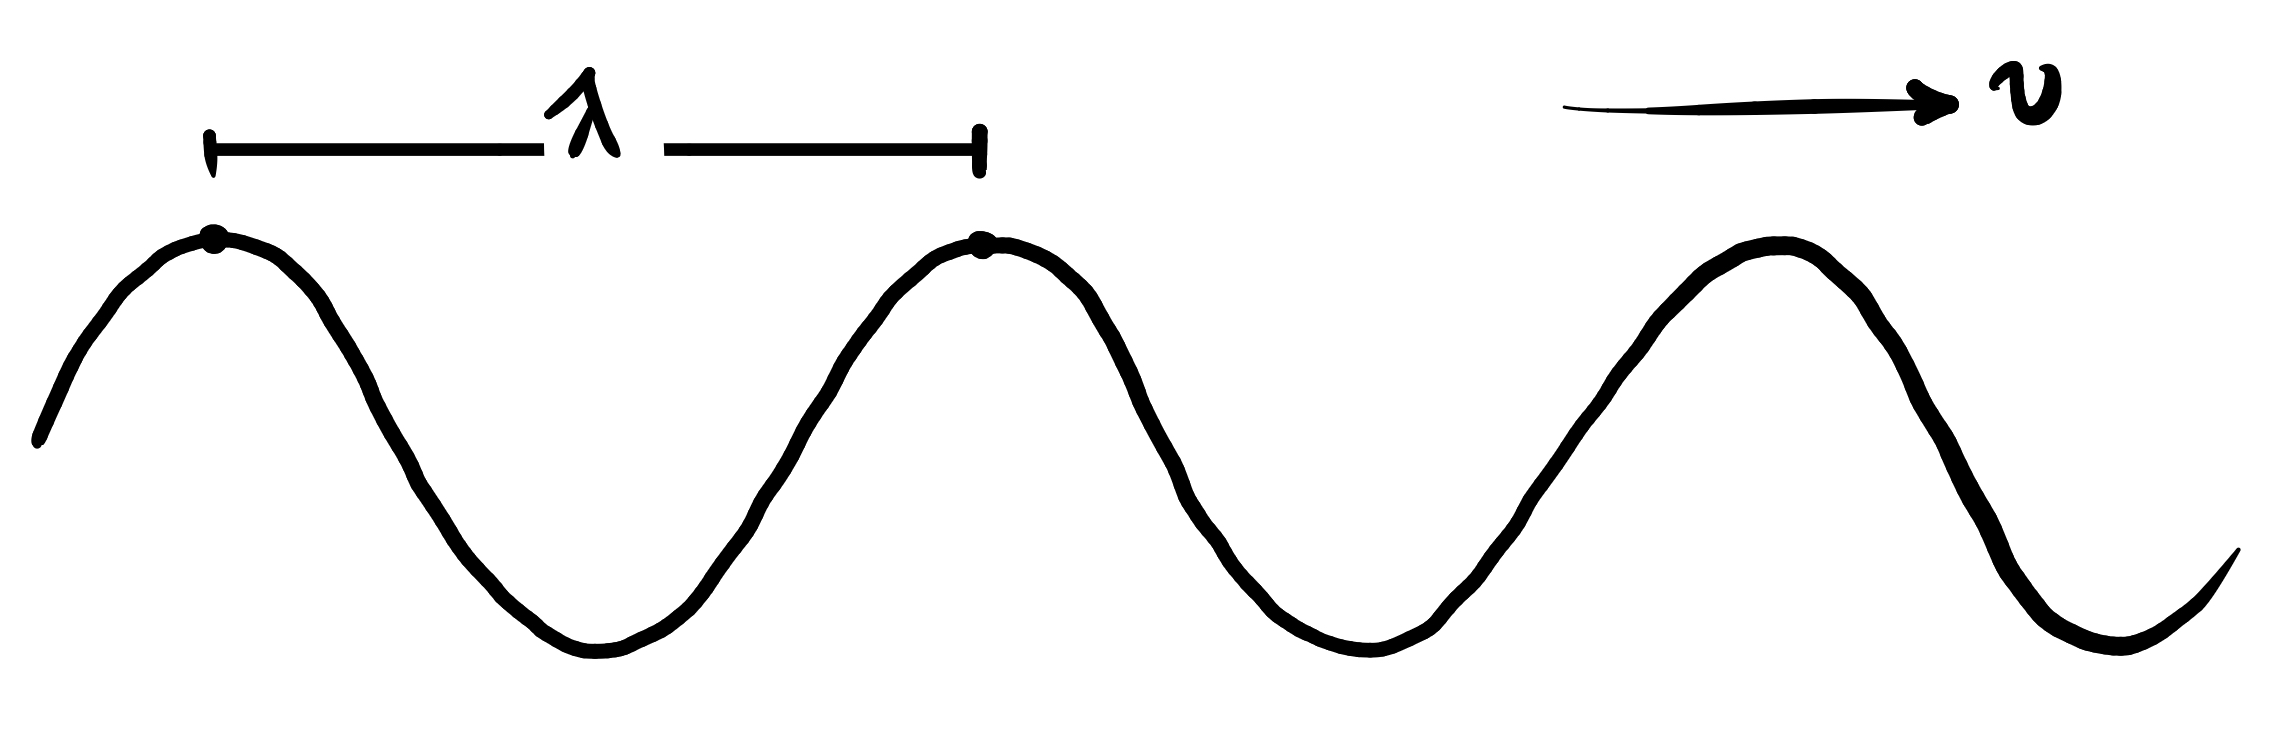
\includegraphics[scale=0.10]{imagensintro/onda.jpeg}};
      \end{scope}
    \end{tikzpicture}
    \caption{Propagação da onda.}
    \label{introonda}
\end{figure}


A Equação \eqref{00intro_eq_vlambdaf} não é resultado de um experimento, tampouco serve para definir alguma grandeza. Ela é uma consequência lógica do que é estabelecido pela teoria. 

Podemos demonstrá-la a partir da equação básica da Cinemática que define a velocidade média --- a Equação \eqref{00intro_eq_velocidade}.


\vspace{0.3cm}
{
\centering
\begin{tikzpicture}
  \begin{scope}[blend mode=multiply]
    \node {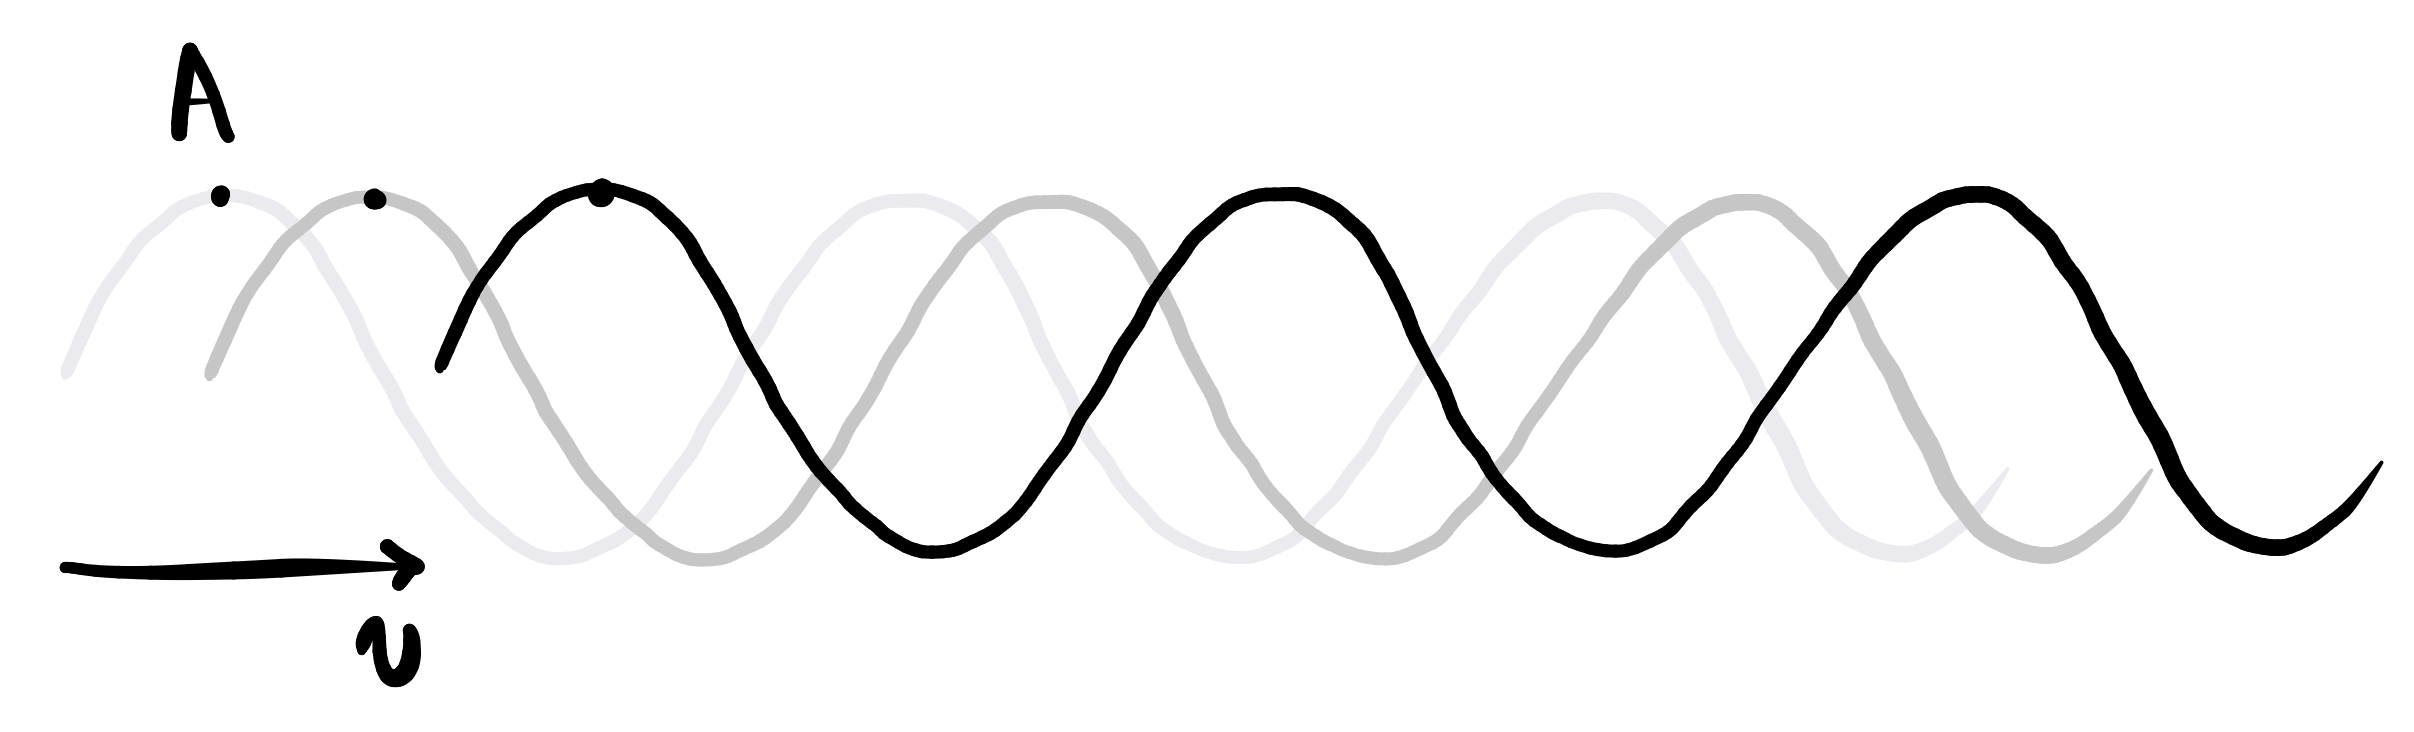
\includegraphics[width=0.8\linewidth]{imagensintro/ondapropagando.png}};
  \end{scope}
\end{tikzpicture}
\captionof{figure}{Onda se propagando para a direita.}
\label{fig_intro_ondapropagando}
} 
\vspace{0.3cm}


A Figura \ref{fig_intro_ondapropagando} mostra diferentes instantes da propagação de uma onda. Observe que o ponto $A$ destacado é sempre o mesmo, ele apenas está representado em diferentes instantes de tempo. Sendo $T$ o tempo de um período (um ciclo da onda) e sendo $\lambda$ definido como a distância que a onda percorre em um ciclo, ou seja, em um período, segue que, ao longo de tal intervalo de tempo, teríamos:

\begin{align}
    d &= vt,  \nonumber \\
    \lambda &= vT, \nonumber
\end{align}
ou seja, no tempo de um período $T$ a distância percorrida será igual a um comprimento de onda, $\lambda.$ Sendo a frequência $f$ dada pelo inverso do período $T$ (outra definição), teremos

$$ \lambda = vT \implies \lambda = v \dfrac{1}{f} \implies \boxed{v = \lambda f.}$$


Ou seja, tal equação é uma verdade fundamental sobre o comportamento das ondas, mas obtida não por meio do experimento, mas sim por meio de explorar a teoria e tentar entender o que decorre logicamente dos seus pressupostos, ou seja, quais são as ``verdades ocultas'', isto é, implícitas, contidas na teoria. Caso o leitor queira entender em um pouco mais de detalhes cada passo lógico usado, fizemos algo como o que segue abaixo:

\begin{quote}
    P1: O comprimento de onda $\lambda$ de uma onda é a distância que tal onda percorre ao longo de um ciclo.\\
    P2: A frequência $f$ de uma onda é dada pelo número de oscilações de tal onda por unidade de tempo.\\
    P3: O período $T$ de uma onda equivale ao tempo para que ela complete um ciclo de oscilação, e é dado pelo inverso da frequência.\\
    P4: A velocidade de propagação da onda é constante, de modo que vale a equação $d=vt.$\\
    C: A onda deve satisfazer a equação $\boxed{v = \lambda f.}$

\end{quote}

O desenvolvimento matemático para se tirar tal conclusão e desaguar na equação destacada é o que foi feito anteriormente.

Faz-se mister destacar ao leitor que a equação $v=\lambda f$ não é a definição de velocidade de uma onda, e sim uma relação que deve ser satisfeita por qualquer tipo de onda, por consequências lógico-matemáticas da forma como se define o comprimento de onda $\lambda$ e a frequência $f.$ A velocidade de uma onda depende, na verdade, das características do meio em que ela se propaga. Por exemplo, para uma onda se propagando em uma corda, sua velocidade é dada pela Equação de Taylor:

$$ v = \sqrt{\dfrac{F}{\mu}},$$

\noindent em que $F$ e $\mu$ representam a tração na corda e sua densidade linear, respectivamente. Estudaremos em detalhes tal equação em um momento futuro. Por hora, é importante notar que, ainda que a velocidade da onda na corda dependa do tipo de corda ($\mu$) e da força de tração na corda ($F$), ela também deve, necessariamente, ser igual ao produto $\lambda f.$ Ou seja, o comprimento da onda naquela corda, sua frequência e a velocidade de propagação dada pela Equação de Taylor devem ser tais que a equação $v=\lambda f$ seja satisfeita.








\section{Um passeio pelas equações}

A introdução feita até aqui é, possivelmente, a parte mais importante de todo este livro. Isso porque, caso o leitor não esteja disposto a ampliar seu horizonte e visualizar as equações matemáticas como informações --- que devem, portanto, ser compreendidas e não meramente memorizadas --- será muito difícil prosseguirmos juntos nessa jornada.

As páginas que se seguem buscarão mostrar todas as equações da Física sob a óptica que apresentamos aqui: vamos entender qual tipo de equação se trata, qual é o papel que aquela equação ocupa e qual é a informação que ela carrega. Em momento algum vamos simplesmente apresentar uma equação, entregar para o leitor um pequeno macete mnemônico para facilitar sua memorização e lhe ensinar como usar a equação para resolver algum problema. 

Eu entendo que, possivelmente, esse tenha sido o caminho trilhado até aqui pelo leitor, mas esse não é um livro que se propõe a fazer mais do mesmo. Se  deseja quebrar esse ciclo vicioso de ``aprendizado'', é preciso que esteja preparado para o momento de ruptura. Dito isso, incentivo o leitor a retornar, caso necessário, nas seções anteriores desta introdução, caso algo não tenha sido bem compreendido. É certo que algumas coisas que discutimos aqui vão se tornar mais claras à medida que avançarmos no texto e aplicarmos tal método em diferentes equações, contudo, é importante que o leitor tenha compreendido o panorama geral antes de iniciarmos este nosso passeio pelas equações da Física.

Parece relevante também comentar a respeito da escolha das equações que serão apresentadas e a ordem em que as apresentaremos. Este é um texto voltado para o estudante do Ensino Médio, de modo que todas as equações que trataremos serão aquelas trabalhadas e apresentadas neste contexto. Além disso, este material não se propõe a esgotar integralmente todas as equações da Física que podem ser estudadas no Ensino Médio: escolhemos, intencionalmente, deixar algumas de fora, a fim de dar espaço para que o leitor possa, posteriormente, por si só, aplicar o método aqui aprendido e construir o entendimento de algumas outras equações. Trabalharemos, portanto, com as principais equações --- as mais clássicas e relevantes de cada tópico --- de modo a passar por todas as áreas da Física, varrendo as suas partes mais relevantes.

Por fim, poderíamos escolher apresentar as equações em blocos de três grupos --- sendo cada grupo um tipo de equação, como enunciamos anteriormente. Contudo, pareceu muito mais didático apresentar as equações organizadas por assuntos, de modo que o texto ficará dividido em três grandes partes:

\begin{itemize}
    \item [(i)] Mecânica.
    \item [(ii)] Óptica, Ondas e Termodinâmica.
    \item [(iii)] Eletromagnetismo.
\end{itemize}

É muito importante que o material seja estudado na ordem cronológica em que é apresentado. Tal ordem foi cuidadosamente escolhida a fim de que cada nova ideia dependa exclusivamente de ideias e conceitos anteriormente construídos. Assim, a experiência e eficiência da aprendizagem será tão mais eficiente quanto mais fiel o leitor se mantiver à ordem de estudos aqui apresentada.

% Este é um material que deve ser usado em paralelo com um curso de Física para o Ensino Médio: quando o leitor estiver estudando, digamos, Hidrostática, ele deve consultar, na parte de Mecânica, a seção sobre tal tema, na qual apresentaremos e destrincharemos as principais equações de tal assunto.

Este material, portanto, não se propõe a ser um material didático completo para se aprender Física, mas sim um material de apoio, que irá apresentar, por uma perspectiva única, as principais fórmulas que se estudam em Física. Na seção sobre Hidrostática, por exemplo, não nos propomos a construir toda a teoria, apresentar todos os conceitos e passar por toda a história de tal tópico. Partiremos da premissa de que isso já foi feito pelo estudante, e, usando tal arcabouço conceitual, vamos apresentar e destrinchar cada equação matemática que se estuda dentro de tal assunto.

Deixamos ao leitor a sugestão de considerar construir tal arcabouço teórico pelo curso Lições de Física, ministrado pelo próprio autor que vos escreve, e disponível na escola on-line Universo Narrado. As próprias seções deste livro foram organizadas com base nos módulos e aulas do curso, de modo a tornar mais fluido e didático o estudo daquele que está fazendo o curso e buscando destrinchar melhor cada fórmula por este material. 



\section{A Mecânica em História}

Como dito, essa é uma coleção que se dividirá em três volumes, sendo este --- o primeiro deles --- sobre Mecânica, e não poderia ser de outra forma.

A mecânica é o ramo da física que estuda como os corpos se movem e por que se movem. Ela busca descrever, por meio de conceitos e fórmulas, as regularidades do movimento dos objetos, desde uma pedra lançada ao ar até o movimento dos planetas. O experimento de se abandonar uma pedra e analisar seu movimento, como fizemos na Figura \ref{intro02}, é algo que a Mecânica se propõe a estudar e analisar.

A Mecânica é uma estrutura conceitual que relaciona:

\begin{itemize}
    \item posição,
     \item tempo,
      \item velocidade,
       \item força,
        \item massa,
         \item momento linear,
          \item torque,
         \item energia.
\end{itemize}


Historicamente, foi o primeiro grande campo da física a adquirir forma matemática rigorosa, sobretudo a partir do trabalho de Galileu e Newton. Por isso, ela serve como porta de entrada natural para o estudo da física como ciência teórica. A maior parte do que se desenvolveu na Física nos três séculos após Newton foi baseada na sua teoria mecânica --- por isso, começaremos por aqui: a base e o alicerce de quase toda a Física.

Neste livro, apesar da sua abordagem, a mecânica não será apresentada como um catálogo de fórmulas, mas como um sistema coerente de ideias, no qual cada equação tem um papel bem definido: algumas introduzem conceitos, outras descrevem regularidades experimentais, e muitas são consequências lógicas dos princípios adotados. Compreender a mecânica é compreender o primeiro grande exemplo de como a natureza pode ser organizada em linguagem matemática.

Mais do que apresentar ao leitor as fórmulas da mecânica, este livro se propõe a contar uma história. A Física, como toda grande narrativa, tem uma estrutura dramática. E se tivéssemos que contar a história da Mecânica --- a maneira como a humanidade aprendeu a descrever o movimento --- ela se desenrolaria naturalmente em três atos.

No \textbf{Primeiro Ato}, aprendemos a \textit{descrever} o movimento. Antes de perguntar por quê os corpos se movem, precisamos ser capazes de dizer, com precisão, \textit{como} eles se movem: onde estão, quão rápido vão, em que direção. É a Cinemática --- a linguagem do movimento, sem julgamentos sobre suas causas.

No \textbf{Segundo Ato}, aprendemos a \textit{explicar} o movimento. Entra em cena a força --- e com ela, Newton. A pergunta já não é apenas \textit{como}, mas \textit{por quê}: o que faz um corpo acelerar, o que o faz parar, o que conserva seu estado. É a Dinâmica --- e com ela surgem também energia, trabalho e impulso, as importantes quantidades conservadas que a natureza parece prezar acima de tudo.

No \textbf{Terceiro Ato}, colhemos os frutos. Com a linguagem e a teoria em mãos, voltamos nosso olhar para o mundo: a gravidade que governa planetas e projéteis, os fluidos que sustentam navios e balões. São as Aplicações --- onde a teoria encontra a realidade e demonstra seu poder.

Três atos, portanto, para contar uma única história: a de como a humanidade aprendeu a ler o livro da natureza. Comecemos, então, nosso mergulho nesse drama.

